\documentclass[pdftex,english,10pt,b5paper,twoside]{book}
\usepackage[T1]{fontenc} % In case we want special characters
\usepackage[utf8]{inputenc} % We are all writing in UTF-8

\usepackage[numbers]{natbib} % We need to tweak our referencing a bit.
\usepackage{appendix} % Fixes formatting of appendices
\usepackage[printonlyused]{acronym} % Package to handle the acronym list
\usepackage{graphicx} % We *may* use images
\graphicspath{{images/}} % and it is clean to put them in a separate dir
\usepackage{amstext} % To support \text in math mode
\usepackage{hyperref} % Internal and external links is nice
\hypersetup{
    pdfborder=0 0 0, % ..especially without red borders
    pdftitle={Cloud Storage Vault},
    pdfauthor={Haver, Melvold and Ruud},
    pdfsubject={Secure Storage in the Cloud},
    pdfkeywords={NTNU, thesis, secure, cloud, cryptographic, sharing}
}

% Packages and settings for code listings
\usepackage{listings}
\usepackage{caption}
\usepackage{upquote}
\usepackage{xcolor}
\DeclareCaptionFont{white}{\color{white}}
\DeclareCaptionFormat{listing}{\colorbox{gray}{\parbox{\textwidth}{#1#2#3}}}
\captionsetup[lstlisting]{format=listing,labelfont=white,textfont=white}
\lstset{
language=Java,
keywordstyle=\bfseries\ttfamily\color[rgb]{0,0,1},
identifierstyle=\ttfamily,
commentstyle=\color[rgb]{0.133,0.545,0.133},
stringstyle=\ttfamily\color[rgb]{0.627,0.126,0.941},
showstringspaces=false,
basicstyle=\small,
numberstyle=\footnotesize,
numbers=left,
stepnumber=1,
numbersep=10pt,
tabsize=2,
breaklines=true,
prebreak = \raisebox{0ex}[0ex][0ex]{\ensuremath{\hookleftarrow}},
breakatwhitespace=false,
aboveskip={1.5\baselineskip},
columns=fixed,
upquote=true,
extendedchars=true,
frame=bottomline,
inputencoding=utf8
}

% Set equal margins on book style
% \usepackage{layout} % Use \layout to print out the margins (debug)
%\usepackage{geometry}
%\geometry{bindingoffset=1cm}
\usepackage[lmargin=25mm,rmargin=25mm,tmargin=27mm,bmargin=30mm]{geometry}

% Restyle chapter headers
\usepackage{fix-cm}
\makeatletter
\renewcommand{\@makechapterhead}[1]{%
  \vspace*{50\p@}%
  {\parindent \z@ \raggedright \normalfont
    \vspace{15pt}%
    \ifnum \c@secnumdepth >\m@ne
        %\hfill\huge\scshape \@chapapp\space
        \hfill\fontsize{60}{90}\selectfont \thechapter % Chapter number
        \par\nobreak
        \vskip 20\p@
    \fi
    \interlinepenalty\@M
    \hfill \Huge \scshape #1\par % Chapter title
    \vspace{5pt}
    \hrule
    \nobreak
    \vskip 40\p@
  }}
\makeatother

\author{Eirik Haver \and Eivind Melvold \and Pål Ruud}
\title{Master thesis - Cloud Storage Vault}
\date{\today}

\begin{document}

\include{title}
\pagestyle{empty}

\chapter*{Abstract}
\addcontentsline{toc}{chapter}{Abstract}
\pagestyle{plain}
\pagenumbering{Roman}
\setcounter{page}{1}

%  Writers should follow a checklist consisting of:
% Motivation: Why do we care about the problem and results?
% Problem Statement: What problem are we trying to solve? Scope/limits.
% Approach: How did we go about solving or making progress on the problem?
% Results: What is the answer? Numbers, not vague 'very', 'small' etc.
% Conclusions: What are the implications of your answer? Further work.
%
%  Each section is typically a single sentence, although there is room for
%  creativity.

Today, major IT-companies, such as Microsoft, Amazon and Google, are offering
storage as a cloud service to their customers. This is a preferable solution to
regular storage in terms of low hardware costs, reliability, scalability and capacity.

However, the idea of storing customer data by an untrusted cloud provider
introduces the issue of data privacy and integrity. The customer is no longer in
position to control the physical access to the stored data, and is therefore
not guaranteed data privacy or integrity by the cloud provider.

To solve this problem, we have proposed a solution that ensures
privacy and integrity of customers' data stored by untrusted cloud providers.
The proposed solution does also support sharing of private data among customers
of the same cloud provider. The solution has further been implemented as a proof of concept. 

When implementing the solution, we first created an underlying framework to support the
proposed and necessary cryptographic functionality. The framework was further
utilized to implement the final application.

Application Results:

Conclusion:


\chapter*{Preface}
\addcontentsline{toc}{chapter}{Preface}

The work behind this project report was carried out during the spring semester
in 2011 at the Norwegian University of Science and Technology (NTNU), Department
of Telematics (ITEM).
\vspace{13pt}

\begin{center}
Eirik Haver, Eivind Melvold and Pål Ruud
\vspace{13pt}

\end{center}

\tableofcontents

\cleardoublepage
\phantomsection
\addcontentsline{toc}{chapter}{\listfigurename}
\listoffigures

\cleardoublepage
\phantomsection
\addcontentsline{toc}{chapter}{\listtablename}
\listoftables

\cleardoublepage
\phantomsection
\addcontentsline{toc}{chapter}{\lstlistlistingname}
\lstlistoflistings
\cleardoublepage

\chapter*{Acronyms}
\addcontentsline{toc}{chapter}{Acronyms}

\begin{acronym}[PBKDF2]
\acro{ACL}{Access Control List}
\acro{AES}{Advanced Encryption Standard}
\acro{API}{Application Programming Interface}
\acro{BFDA}{Brute Force and Dictionary Attack}
\acro{CA}{Certification Authority}
\acro{CBC}{Cipher Block Chaining}
\acro{CDA}{Cluster Dictionary Attack}
\acro{CG}{Credential Generator}
\acro{CPU}{Central Processing Unit}
\acro{CSV}{Cloud Storage Vault}
\acro{DP}{Data Processor}
\acro{DRY}{Don't Repeat Yourself}
\acro{DSA}{Digital Signature Algorithm}
\acro{DSS}{Digital Signature Scheme}
\acro{DV}{Data Verifier}
\acro{EC2}{Elastic Compute Cloud}
\acro{ECB}{Electronic Codebook}
\acro{FAQ}{Frequently Asked Questions}
\acro{GPU}{Graphics Processing Unit}
\acrodef{GUI}{Graphical User Interface}
\acro{FEC}{Forward Error Correction}
\acro{HDFS}{Hadoop Distributed File System}
\acro{HTTP}{Hypertext Transfer Protocol}
\acro{HTTPS}{Hypertext Transfer Protocol Secure}
\acro{IaaS}{Infrastructure as a Service}
\acro{IV}{Initialization Vector}
\acro{JCA}{Java Cryptography Architecture}
\acro{JCE}{Java Cryptographic Extensions}
\acro{JDK}{Java Development Kit}
\acro{JRE}{Java Runtime Environment}
\acro{JVM}{Java Virtual Machine}
\acro{LAFS}{Least Authority File System}
\acro{MAC}{Message Autentication Code}
\acro{MITM}{Man-in-the-middle}
\acro{NIST}{National Institute of Standards and Technology}
\acro{OS}{Operating System}
\acro{PBKDF2}{Password-Based Key Derivation Function version 2}
\acro{PaaS}{Platform as a Service}
\acro{PasS}{Privacy as a Service}
\acro{PEP}{Python Enhancement Proposal}
\acro{PGP}{Pretty Good Privacy}
\acro{PKI}{Public Key Infrastructure}
\acro{PoC}{Proof-of-concept}
\acro{PRNG}{Pseudorandom Number Generator}
\acro{QR}{Quick Response}
\acro{RAM}{Random Access Memory}
\acro{ROM}{Read Only Memory}
\acro{REST}{Representational State Transfer}
\acro{RSA}{Rivest, Shamir and Adleman}
\acro{SaaS}{Software as a Service}
\acro{SDK}{Software Development Kit}
\acro{SHA}{Secure Hash Algorithm}
\acro{SQL}{Structured Query Language}
\acro{SSL}{Secure Socket Layer}
\acro{TCCP}{Trusted Cloud Computing Platform}
\acro{TCG}{Trusted Computing Group}
\acro{TG}{Token Generator}
\acro{TLS}{Transport Layer Security}
\acro{TPM}{Trusted Platform Module}
\acro{TTP}{Trusted Third Party}
\acro{UMTS}{Universal Mobile Telecommunications System}
\acro{URI}{Uniform Resource Indetifier}
\acro{URL}{Uniform Resource Locator}
\acro{USB}{Universal Serial Bus}
\acro{VM}{Virtual Machine}
\acro{WSGI}{Web Server Gateway Interface}
\end{acronym}

%**************************************%
\chapter{Introduction}
%**************************************%
\pagenumbering{arabic}
\setcounter{page}{1}

% TODO: Generic introduction 

The term \emph{Cloud Computing}, and the common shorthand \emph{The Cloud},
is not yet clearly defined \cite{clouddef}, but involves the provision of
software or computational resources available by demand via the Internet.
In a draft \cite{cloud_nistdef}, the \ac{NIST} defines cloud computing as:
\begin{quote}\it
``Cloud computing is a model for enabling ubiquitous, convenient,
on-demand network access to a shared pool of configurable computing resources
(e.g., networks, servers, storage, applications, and services) that can be
rapidly provisioned and released with minimal management effort or service
provider interaction.''
\end{quote}

More and more of the traditionally locally hosted services of businesses is
moving to the cloud. The amount of flexibility and cost savings this
provides, can be quite extensive.

Today, we take the services that the established cloud providers offer us for
granted. For example, both Google and Microsoft provides the services of online
document editing, email, picture collections, file storage and a lot more for
free, and available at anytime from anywhere \cite{googleservices,
microsoftservices}.

However, this often comes at a cost of reduced privacy, as the control over the
hosting environment is lost. Users is therefore forced to increasingly think
about how the data stored online can leak to unwanted people, either by
accident, or by purpose by unfaithful servants at the cloud provider. Should it
be sufficient to trust the security policies of the cloud providers, or is it
possible to handle the privacy issues locally before giving away the files?

\section{Motivation}

In the last decade, the available supply for services that offer data storage
remotely in the cloud has increased considerable. Storing private data at a
third party provider, in contrast to self-hosted storage devices, has proven to
be preferable due to low storage costs and high reliability, scalability and
capacity.

However, storing data at a remote location prevents users from physically
protecting their storage medium. With this in mind, there is no guarantee that
a customer's data is kept private and secure from disloyal employees at the
storage provider.

To solve this issue, there has lately been introduced numerous applications and
architectures \cite{dropbox_security, tahoe, tccp, PasS} providing solutions to
ensure privacy and integrity of customer data stored at the \emph{insecure}
cloud provider. However, all of these alternative systems are missing one
or more features towards being, as we will define it, a completely secure
storage solution.

This situation has given motivation to implement a proof of concept
application, that fulfills all of the criteria for what we define as a secure
cloud storage service.

Additionally, we do also see this as a golden opportunity to learn more
about software development, development methodologies, team work, and practical
use of information security and cryptography.

\section{Related Work}

In the later years, there has been quite a lot of research done in the field of
security in cloud computing. The problems that arise, are fundamentally not
different from those revealed by classic information security scenarios. The
key point, is that when using a service hosted by someone you do not know if
you can trust, you have to treat that \emph{someone} as untrusted and as a
possible attacker. Generally speaking, you loose control over the hosting
environment, and hence has to deal with the security issues this implies.

In Section \ref{sec:research}, we present four papers \cite{PasS,
privacymanager, tccp, microsoftresearch} which try to solve security issues in
a shared hosting environment. Common to all of these, is that they either rely
on special, secure and tamper-proof hardware and/or a trusted third party.

Another way of providing a solution to the same problem, is to give the
responsibility of the security operations to the client, i.e. in an environment
that the user has control of. In Section \ref{sec:existing}, we present three
commercially and publicly available software services that relates to this way
of thinking.

One of these applications, Tahoe-\ac{LAFS} \cite{tahoe}, is given special
attention. This is because it is an Open Source and a well documented piece of
software, that answers most of the problems arising in an untrusted cloud
storage environment, and relates closely to the work performed in this thesis.

\section{Scope and Objectives}

There are two main objectives of this thesis. The first objective is to create a
cryptographic scheme that can provide secure storage of data by using an untrusted
cloud storage provider. We define secure storage by the following criteria.
\label{sec:criteria}
\begin{enumerate}
  \item Data should be encrypted in a safe environment trusted by the owner,
  before it is stored.
  \item It should be possible to verify the integrity of the stored data.
  \item Only authorized people should have access to the data.
  \item The storage scheme should be documented in detail, such that users can
  easily understand the scheme and accept/reject it on that basis. 
  \item An implementation of the storage scheme should be Open Source.
\end{enumerate}

The cryptographic scheme should, in addition to the mentioned security, provide
the possibility of sharing stored data between multiple cloud storage customers. The security
requirements above should also be valid for the shared data. The underlying scheme for
sharing data should be applicable for both enterprise and regular customer
scenarios.

The second main objective is to implement the proposed scheme as part of a
proof of concept application for Android devices. The application should be
designed for regular customers, although the underlying cryptographic scheme
should additionally support enterprise scenarios. It is further important that the server side of the
application is compatible with as many existing cloud storage providers as possible.
%This will require the application to only
%utilize known standard components, such as the HTTP protocol and the TLS channel.

Finally, it is important that the implementation of the cryptographic scheme
is available as Open Source.

\section{Limitations}

We will focus on making an architecture that covers the scope and objectives,
in an easy to understand and complete way. In addition, making core
functionality, that demonstrates the most important security features in a proof
of concept system, will be prioritized.

However, due to time and resource constraints, we will focus less on the following:
\begin{itemize}
  \item The language in the proof of concept client should be clear, but the
    \ac{GUI} in itself will not get special attention
  \item Experimentation with the proof of concept code, other
    than basic performance and security measurements
  \item Experimentation with the proof of concept client on hardware equipment
    other than what we easily have available at the time of testing
\end{itemize}

\section{Methodology}

The work behind this thesis, is carried out by the three authors in
cooperation. The methodology used, can be categorized based on the three main
parts of this work; the \emph{research}, the \emph{design and abstraction}
part, and the \emph{software development} cycles.

The research will include an analysis of related systems, and a study of
relevant background theory. Based on this theory, we will use experimentation
to create and design a theoretical solution to the problem of secure storage
and sharing of files on an untrusted server. We will iteratively analyse our
experimentation to find and correct flaws with the design.

The third part of the work, is the software development cycles of the proof of
concept application. 

\paragraph{SCRUM} We will work after SCRUM principles -- an iterative and
incremental based framework for project management \cite{scrum}. There does not
exist a SCRUM \emph{product owner} for the system we will create, nor do we
fulfill the requirements and characteristics \cite{scrum} of a traditional
SCRUM \emph{team}. Hence, we will use the principles that are practically
possible for us to follow:

\begin{itemize}
  \item Daily \emph{stand-up} with planning of the tasks of the current day
  \item Weekly \emph{sprint}\footnote{A \emph{sprint} is a defined period with
    a given set of tasks.} planning meetings 
  \item Keep tasks on stickers, that we move between different phases on a
    board: \emph{to do}, \emph{in progress}, \emph{quality assurance} and
    \emph{done}. This is to keep track of progress in the current sprint
  \item Continuously analyse the process, and improve it if possible
\end{itemize}

\paragraph{DRY} We choose to follow the \ac{DRY} principle when developing
software. \citet{dry} define \ac{DRY} as:

\begin{quote}\it
Every piece of knowledge must have a single, unambiguous, authoritative
representation within a system.
\end{quote}

\noindent This principle can be taken further, as to not develop something that
has already been developed in the past. If there exist a library for a given
task that does fulfill the requirements set for the specific task, we will
choose to utilize the library instead of developing similar code by ourselves.

\section{Outline}

This thesis is presented as per the following chapters:

\paragraph{Chapter \ref{ch:background} -- Background} provides background
knowledge of the security services, technologies and software used to form a
secure cloud storage system. In addition, relevant research and commercial
solutions are scrutinized.

\paragraph{Chapter \ref{ch:technical} -- Technical Procedure} goes through the
development process of the scheme and software produced by this thesis. It
starts with an overview of the architectural properties, followed by the more
specific cryptographic scheme that fits in with the architecture. Lastly, the
implementation of the proof of concept system is described.

\paragraph{Chapter \ref{ch:experimental} -- Experimental Procedure} presents
the measurements and practical experimentation done to look at how the system
performs performance- and security-wise.

\paragraph{Chapter \ref{ch:results} -- Results} illustrates the findings from
the experimentation.

\paragraph{Chapter \ref{ch:discussion} -- Discussion} reflects on the specific
implementation and results from the previous chapters. In addition, associated
functionality to a secure cloud storage system, that has not been mentioned
earlier, is presented and discussed.

\paragraph{Chapter \ref{ch:conclusion} -- Conclusion} extracts the most
important results and findings, and concludes the work done in this thesis.
Further work that can be applied to the created system and scheme,
are prioritized and presented as final ideas.

\bigskip

\noindent In addition, included appendices consist of:

\paragraph{Appendix \ref{ap:other} -- Other Relevant Implementations}
presents the implementations created to carry out the security experiments.

\paragraph{Appendix \ref{ap:attachments} -- Attachments} describes the contents
of the supplied attachments provided.

%**************************************%
\chapter{Background}
\label{ch:background}
%**************************************%

The basis and underlying technologies for a secure storage service in the
cloud, are quite numerous and quite often complex.

In the following sections, we will go through the security services, cryptographic
services and attacks that are relevant to such a service. In addition, we present
related research and existing solutions available at the time of writing.

This chapter forms the basis for the architecture of the proposed solution
presented in this thesis.

\section{Security Services}

This section explains the security services and technology used in this thesis. A security
service is any processing or communication service that enhances the security of
the data processing systems and the information transfers of any organization,
as defined by \citet[p. 12]{stallings}.

\paragraph{Confidentiality} Confidentiality is the act of keeping a message
secret from unauthorized parties \cite[p. 18]{stallings}. This can typically be
done by either preventing other parties access to the message at all, or by making
the contents unreadable, for instance by the use of encryption.

\paragraph{Integrity} Integrity implies that a message cannot be altered
without the receiving part noticing. In a security perspective, integrity deals
with detecting, preventing and recovering a message being changed by an
attacker \cite{stallings}.

\paragraph{Availability} The property of a system being accessible and usable
upon demand by an authorized system entity, are defined by the availability
service \cite{stallings}.

\paragraph{Authentication} Authentication is the act of a user, service or
similar to prove that he is what he claims to be \cite{stallings}.

\paragraph{Non-Repudiation} Non-repudiation prevents both the sender and the
receiver of a message from refuting the authenticity of transmitted message. In
other words, one party can prove the involvement of the other party
\cite{stallings}.

\section{Cryptographic Primitives}

This section describes the low level security primitives used in the results of
this thesis.

\emph{Randomness} is a basic property that multiple of the cryptographic
primitives rely on, and hence deserves an explanation. Random data is
informally defined as unpredictable to the attacker, even if he is taking
active steps to defeat the randomness \cite[p. 137]{schneier}.

A \emph{Cryptographic \ac{PRNG}} deterministically produce numbers based on a
seed, and it should be infeasible to determine the next number without knowing
the seed \cite[p. 140]{schneier}.

\subsection{Encryption}

Encryption is the process of transforming some information into an unreadable
form. It is primarily used to enforce confidentiality, but can also be
used for other purposes, e.g. authentication.

In its very basic form, an encryption scheme consist of an encryption algorithm
(the \emph{cipher}), a key and a message (the \emph{plaintext}), that is all
used to create an encrypted message, i.e. the \emph{ciphertext}. If a strong
cipher is used, knowledge of the cipher, or multiple plaintext and multiple
ciphertext, should not be enough to obtain the key, or to decrypt ciphertext
with a corresponding unknown plaintext \cite{schneier}.

\paragraph{Block Cipher and Stream Cipher} There are different classifications
on how a cipher treats data \cite[p. 32]{stallings}. A \emph{block cipher} will
encrypt a block of data of a specific size. If the data is larger than the
block size used by the application, a \emph{mode of operation} is needed. In a
\emph{stream cipher}, the plaintext will usually be combined with a pseudorandom key
stream to generate the ciphertext.

\paragraph{Symmetric Encryption} Symmetric-key encryption is an encryption scheme
where the same key is used for both encryption and decryption \cite[p.
32]{stallings}. The \ac{AES} is a block cipher and is the current standard for
symmetric encryption. The \ac{AES} works on a block of 128 bits at a time,
and support keys with length of 128, 192 and 256 bits.

\paragraph{The Mode of Operation} The mode of operation used for a
symmetric-key encryption enables subsequent safe use of the same key.

In a simple scenario, this could be to encrypt the normal data block-by-block
with pure \ac{AES}, which is called the \ac{ECB} mode of operation. The problem
with this is that some information of the plaintext will leak, i.e. the same
plaintext will always be encrypted as the same ciphertext.

An other mode is \emph{\ac{CBC}}. In \ac{CBC}, a non-predictable and not reused
\ac{IV} is used. The \ac{IV} is XORed with the first block of plaintext, which
again is encrypted with \ac{AES}. The resulting ciphertext is used as an
``\ac{IV}'' for the next block \cite[p. 183]{stallings}, and so on.

\paragraph{Asymmetric Encryption} Asymmetric key encryption is an encryption scheme
where different keys are used for encryption and decryption
\cite[p. 259]{stallings}.

An asymmetric encryption scheme is often called a \emph{public-key
encryption} scheme, where one key is defined as private and the other as public.
The public key is shared to allow other parties to encrypt messages that only the
owner of the private key can decrypt.

The downside of asymmetric encryption compared to symmetric is that it requires
a larger key, and that it has a larger computational overhead to obtain the
same level of confidentiality as comparable symmetric-key encryption. The
probably best known asymmetric cipher is \ac{RSA}.

\subsection{Cryptographic Hash Functions}

A cryptographic hash function is a deterministic mathematical procedure, which
takes an arbitrary block of data and outputs a fixed size bit string. The
output is referred to as the \emph{hash value}, \emph{message digest} or simply
\emph{digest}.

Another property of a cryptographic hash function, is that the
smallest change in the input data, e.g. one bit, should completely change the
output of the hash function. In other words, it should be infeasible to find the
reverse of a cryptographic hash function \cite[p. 335]{stallings}. It should
also be infeasible to find two blocks of data which produce the same hash value
(a \emph{collision}).

The standard for cryptographic hash functions today, are \ac{SHA}-1 and the
\ac{SHA}-2 family.

\section{Applications of Cryptographic Primitives}

\subsection{Digital Signatures}

A digital signature is the digital equivalent of a normal signature, i.e. it
verifies that an entity approves with or has written a message. It can also
verify the date the signature was made. In addition, it should be verifiable by
a third party \cite[p.  379]{stallings}.

It should logically not be possible, or at least unfeasible, to fake a digital
signature.

The \ac{RSA} cipher can be used to generate signatures. In addition, there is also a
standard for digital signatures, called \ac{DSS}, which uses \ac{DSA} as the
underlying algorithm.

\subsection{Digital Certificates and PKI}

A digital certificate is the pairing of a digital signature and a public key
\cite{stallings}. By this scheme, the services confidentiality, authentication
and non-repudiation can be achieved.

For example, a person has a certificate with some clues about the identity
in it, e.g. the e-mail, together with a public key. This certificate can then
be signed using digital signatures, to verify that some other entity trusts this
certificate.

In practice, the entity which signs certificates is the \ac{CA}, which all
clients have the public key information for, and trusts. The \ac{CA} will also
contain information about which certificates has been revoked, i.e. should not
be trusted in use. Such a scheme is usually referred to as a \ac{PKI}.

\subsubsection{PGP}

\ac{PGP} is a scheme similar to \ac{PKI}, but with no \ac{CA} that all users
trust \cite{stallings}. Instead, trust is made between users by somehow
verifying their public key, for instance by meeting face to face. A user can
then sign another users key, set a trust level for the user, and publish this
information to a key server.

Another user can then calculate a trust on an unknown person, based on the trust
set by peoples that he trusts, from information located on publicly
available key servers.

\subsection{SSL/TLS}

\ac{TLS}, and its predecessor \ac{SSL}, are technologies for obtaining
confidentiality, integrity and authentication for transfer of files over a
network \cite{stallings}. It does so by a combination of different algorithms
and primitives, but a digital certificate is required for authentication.

To transfer files securely over \ac{HTTP}, \ac{TLS}/\ac{SSL} is used to form
\ac{HTTPS}.

\subsection{PBKDF2}
\label{sec:PBKDF2}

\ac{PBKDF2} is a key derivation function used to create an encryption key based
on a password. The key point of this, is that a password is often something
that a person has to be able to recall from memory. But, a password phrase that
is memorable to a person, might be too short to withstand a dictionary or even
a brute force attack.

What \ac{PBKDF2} does, is to make the process of deriving the key from the password
an expensive process in terms of computational power, to make it more resistant
to brute force attacks. This feature is known as \emph{key stretching}.

The efficiency of the key derivation, is dependent on the number of process
iterations chosen in the implementation of the function.

\section{Security Attacks}

This section briefly list security attacks relevant to this thesis, as defined
by \citet[Ch. 1.3]{stallings}.

\paragraph{Active and Passive Attacks} Two general classifications of security
attacks exist, where a \emph{passive attack} attempts to learn or make use of
information from the system, but does not affect system resources. An
\emph{active attack} attempts to alter system resources or affect their
operation.

\paragraph{Traffic Analysis} Traffic Analysis is the act of capturing and
examining communication data sent between two parties. This information might
contain secrets or for instance leak enough information about an encryption key
to make it breakable.

\paragraph{Masquerade} Masquerade is an active attack where the attacker pretends to be
one of the legitimate parties.

\paragraph{Replay} Replay is an active attack where the attacker capture some
data in a communication session and subsequently retransmit that information.

\paragraph{Modification of Messages} Modification of messages is an active
attack where the attacker alters some of the contents of a message sent between
two communicating parties.

\paragraph{Denial of Service} Denial of Service is an active attack where the
attacker seeks to make resources unavailable for legit users, i.e. by
overloading an application by sending it lots of traffic.

\paragraph{\acl{MITM}} \ac{MITM} is an attack where an attacker intercepts messages
between the communicating parties and then either relay or substitute the
intercepted message.

\subsection{Attacks on Cryptographic Primitives}

Even though cryptographic primitives are designed to be secure, they might have
implementation flaws and be used in an improper fashion, e.g. by using wrong
parameters.

\paragraph{Cryptanalysis Attack} A cryptanalysis attack is an attempt to deduce
a specific plaintext or to deduce the key being used in a ciphertext.

\paragraph{Brute-Force Attack} In a brute-force attack, an attacker tries
to obtain a secret by testing the algorithm with up to all possible inputs. The
secret might be an encryption key, or the data fed into a cryptographic hash
function.

A related attack is the \emph{Dictionary attack}, where the attacker
tries to obtain a secret by trying a subset of all known inputs, i.e. a
predefined dictionary of words.

\section{Cloud Computing}

In this section, we will extend from the definitions given in Section
\ref{sec:intro:intro}, and further describe terms that are associated with
\emph{Cloud Computing}.

\subsection{Service Models}
The \ac{NIST} also defines three service models which deals with what kind of
service the consumer can rent from a provider.

\paragraph{\ac{SaaS}} The capability for a consumer to run the provider's
application running on cloud infrastructure, using a thin-client, browser or
similar, is called \ac{SaaS}. The web-based email service
GMail\footnote{\url{http://www.gmail.com}} can be seen as an example of this.

\paragraph{\ac{PaaS}} The capability for a consumer to deploy software onto
the cloud, but without actually controlling the underlying platform, operating
system and so on, is called \ac{PaaS}.

\paragraph{\ac{IaaS}} The capability provided to the consumer to provision
processing, storage, networks and other fundamental computing resources where
he can run arbitrary software, including operating systems and applications, is
called \ac{IaaS}. An example is when renting a \ac{VM}.

\subsection{Deployment Models}

The \ac{NIST} draft \cite{cloud_nistdef} also lists several deployment models
which deals with how the cloud is organized in terms of where it is hosted, and
who has access to it.

\paragraph{Private Cloud} A private cloud is a cloud infrastructure operated
solely for an organization. Which party manages the cloud, and where it is
located is not defined.

\paragraph{Community Cloud} A community cloud is a cloud infrastructure is
shared by several organizations to serve a common concern. Where it is located
and who manages it is not given.

\paragraph{Public Cloud} A public cloud is a cloud infrastructure where
everyone, or at least a large group, can have access, and is owned by an external
provider of cloud services.

\paragraph{Hybrid Cloud} A hybrid cloud is a cloud infrastructure composed of
two or more clouds of any other model.

\subsection{Security Considerations in Cloud Computing}

There are some considerations when using cloud services from an external
provider, as opposed to self controlled hardware, software and platforms. Most
notably is that you loose the control of selecting the people which will have
physical and digital access to the infrastructure \cite{cloud_getoff}. In
essence, this means that the provider can read every data sent to and from the
cloud as well as the data saved in the cloud.

Another risk is that information might be leaked to other users of the same
cloud. For instance it might be able possible for a \ac{VM} to leak information
to other \acp{VM} on the same host \cite{cloud_getoff}.

\section{Research}
\label{sec:research}

This section will elaborate on selected previous research concerning privacy
within cloud computing. The research on this subject can be divided into
proactive solutions that either reduce, or prevent the risk of leaking privacy
related information. Only the latter type of solutions are further discussed.

\subsection{Privacy as a Service}

A concept entitled \ac{PasS}, was suggested in 2009 \cite{PasS}. \ac{PasS} is a set
of security protocols ensuring privacy of customer data in cloud computing
architectures. The main design goal with \ac{PasS}, is to maximize the user's control
over his sensitive data, both processed and stored within a cloud.

The \ac{PasS} concept is based on a fundamental \emph{system model} and \emph{trust
model}. The system model consists of three communicating parties, namely a
\emph{cloud provider}, a \emph{cloud customer} and a \emph{\ac{TTP}}. The
\ac{PasS} system model is shown in Figure \ref{fig:RW:PasS}.

\begin{figure}[h!]
    \centering
    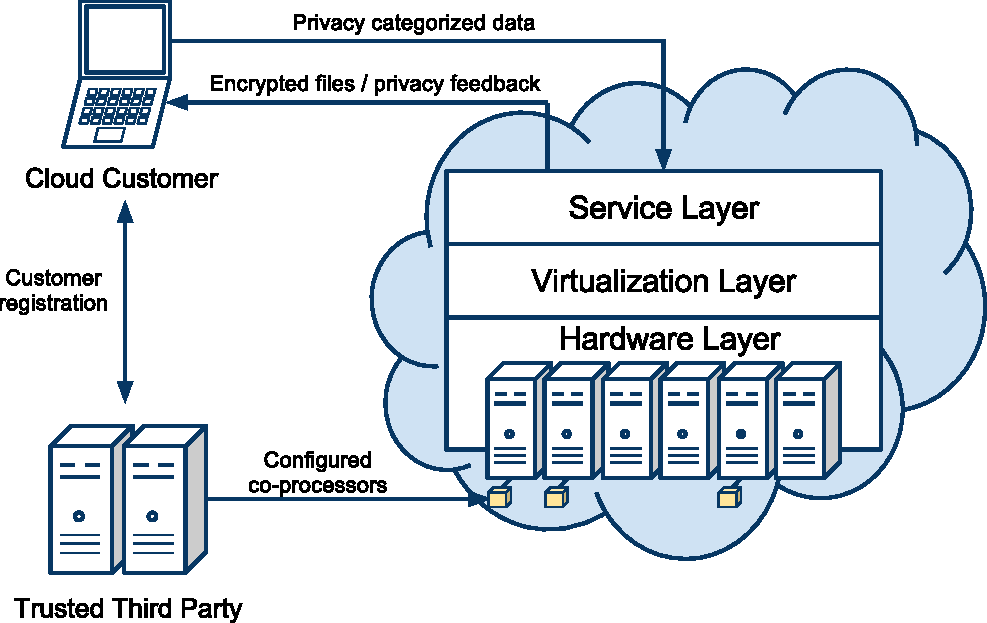
\includegraphics[scale=0.6]{ArchitecturePasS.pdf}
    \caption{System model of PasS}
    \label{fig:RW:PasS}
\end{figure}

It is important to notice that the \ac{PasS} system model is dependent on
pre-installed cryptographic coprocessors in the hardware running the cloud
service.

A cryptographic coprocessor is a small hardware card, including a processor,
\ac{RAM}, \ac{ROM}, backup battery, persistent storage and an Ethernet network
card. A coprocessor interfaces with a server in the cloud, and provides a safe
environment for processing of a customer's sensitive data.

The cryptographic coprocessors are used in the cloud because they are
tamper-proof against physical attacks. The coprocessors are pre-configured by
the \ac{TTP} before they are installed. By using this procedure, the \ac{TTP}
provides a safe computational environment for the cloud customer, which is kept
secret from the cloud provider.

The main task of the \ac{TTP} is to compute a set of public/private key pairs,
load them into the persistent storage of the co-processor, and further send
them to the customer. The \ac{TTP} also loads its own secret key into the
coprocessor. This key distribution ensures secure communication between the
\ac{TTP}, coprocessors and the cloud customer. The customer's key pair is sent
through a secure communication channel.

With cryptographic coprocessors in the cloud and a secure communication, the
cloud customer can choose between three different levels of privacy towards the
cloud provider -- no privacy, privacy with a trusted provider and privacy with
a none-trusted provider.

\emph{No privacy} implies storing data as clear text in the cloud.
\emph{Privacy with a trusted provider} involves storing encrypted data in the
cloud. This data is encrypted by the cloud provider and only achievable by the
customer or cloud provider.

In the case of \emph{privacy with a non-trusted provider}, the customer
encrypts the private data before uploading it to the cloud provider. The key
used for encryption is shared with the cryptographic co-processor, through an
authenticated version of the Diffie-Hellman key management protocol. The
co-processor can further process the encrypted data and store it in the cloud
facility. The stored data is encrypted and unknown to the cloud provider.

\subsection{Privacy Manager}

In 2009, HP Labs proposed a way to manage and control a user's private data,
stored and processed in a cloud facility \cite{privacymanager}. Their solution
was partially implemented as a software program called a \emph{privacy manager}.

The privacy manager uses a feature called \emph{obfuscation}, which is quite
similar to encryption. However, the obfuscation method is different from
encryption in the sense that the obfuscated data can be processed in the
cloud, without the cloud provider knowing the encryption key or the original
data. \citet{privacymanager} mention the following obfuscation methods:

\begin{itemize}
\item Yao's protocol for secure two-party computation \cite{yao}
\item Gentry's homomorphic encryption scheme \cite{gentry}
\item Narayanan and Schmatikov's obfuscation method \cite{obfuscationmethod}
\end{itemize}

Due to better efficiency, the privacy manager uses the latter alternative. However,
Narayanan and Schmatikov's obfuscation method does not provide complete
confidentiality to the cloud provider \cite{obfuscationmethod}.

In addition to installing a privacy manager at the user's terminal, HP Labs
suggests the use of trusted computing solutions to address the lower-level
protection of data. The \ac{TCG} is an example of an organization developing
and providing trusted computing solutions \cite{tcg}. A tamper-proof piece of
hardware called a \ac{TPM} is recommended \cite{privacymanager}, which is
designed by \ac{TCG}. The \ac{TPM} is installed in the machine running the
privacy manager, to ensure that processes carried out by the privacy manager can
be fully trusted.

The privacy manager is suggested to work in three different use cases. It can
be implemented to support a \emph{single client}, the use of \emph{hybrid
clouds} and/or the use of an \emph{infomediary} within the cloud.

%Regarding applications in the cloud where users have to upload unobfuscated
%private data, the privacy manager includes two additional features called
%preferences and personae. Both features are dependent on a trustworthy service
%and cloud provider, and are therefore irrelevant to our development.

\subsection{Trusted Cloud Computing Platform}

Equal to \acl{PasS} and the privacy manager, \emph{\ac{TCCP}} was proposed as a
solution to provide secure computations and storage within a non-trusted cloud
provider \cite{tccp}. As opposed to the previous solutions, \ac{TCCP} is
directed against secure execution of guest \acp{VM} outsourced to \ac{IaaS}
providers.

The original infrastructure, before adding \ac{TCCP}, is assumed to
consist of a \emph{cloud manager}, which manages a cluster of nodes running one or more
\acp{VM}. Among multiple tasks, the cloud manager is responsible for loading \ac{VM}
images into its own nodes.  Each node has a \emph{\ac{VM} monitor} which will further
launch and monitor \acp{VM} from the received corresponding images.

\ac{TCCP} is based upon the \acf{TPM} chip designed by the \acl{TCG}. The
\ac{TPM} contains a private/public key pair that it uses to uniquely identify
itself. The public key is additionally signed by the manufacturer to guarantee
correctness of the \ac{TPM} chip.

With this in mind, \ac{TCCP} is based upon a \emph{remote attestation scheme}.
The scheme enables a network entity to verify whether another remote entity
runs a \ac{TPM} chip or not. A detailed description of the remote attestation scheme
is given by \citet{tccp}.

The \ac{TCCP} system architecture is illustrated in Figure \ref{fig:RW:TCCP}.
The trusted computing base of \ac{TCCP} includes a \emph{trusted coordinator}
and a \emph{trusted virtual machine monitor}. The coordinator manages the
trusted nodes within a cluster. To be trusted, a node must be located within a
security perimeter and run a trusted virtual machine monitor.

\begin{figure}[h!]
    \centering
    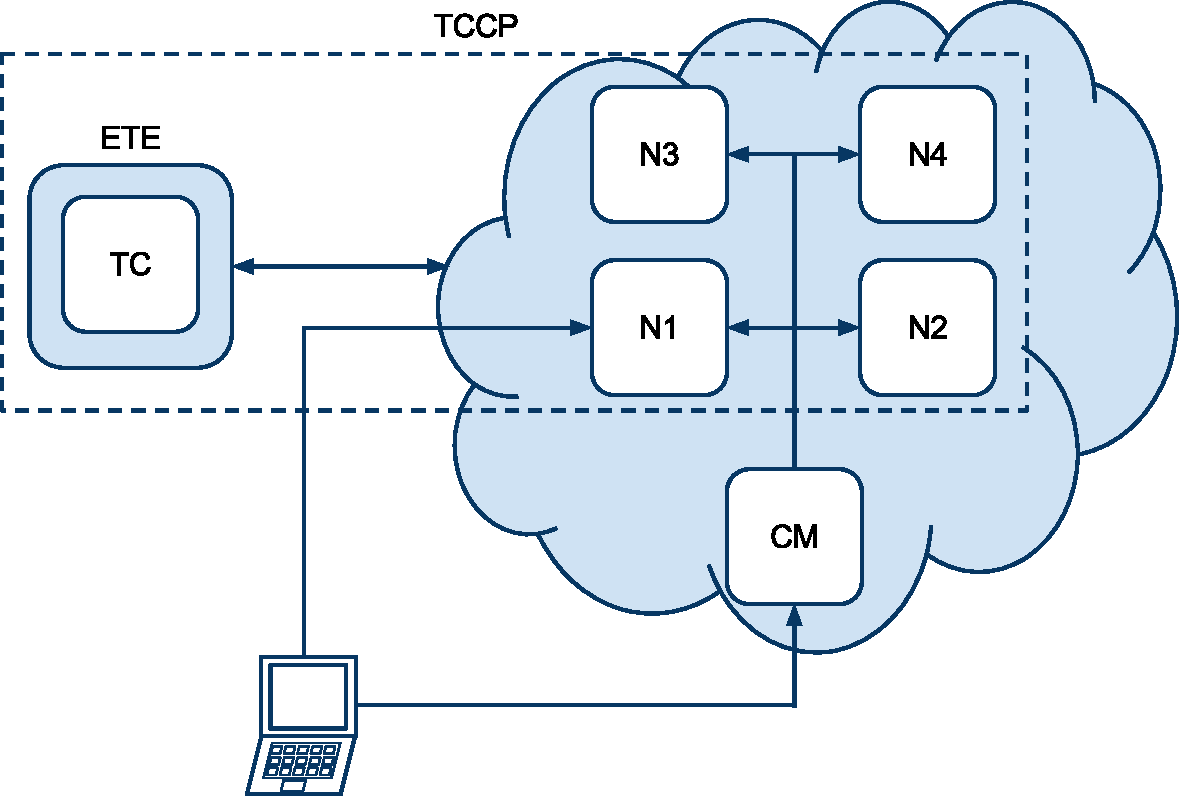
\includegraphics[scale=0.4]{ArchitectureTCCP.pdf}
    \caption{System architecture of TCCP}
    \label{fig:RW:TCCP}
\end{figure}

The coordinator maintains a record of the nodes located in the security
perimeter, and use remote attestation to ensure nodes are trusted. Each trusted
node in a cluster contains a \ac{TPM} chip and a corresponding trusted monitor.
The main task of the trusted monitor, is to enforce a local closed box
protection of a client's running \ac{VM}. Details about the design of the
trusted \ac{VM} monitor, are given by \citet{tccp}.

Each trusted virtual machine monitor cooperates with a trusted coordinator to
protect the transmission of \acp{VM} between trusted nodes, and to ensure that
\acp{VM} are executed by trusted nodes. In this context, the \ac{TCCP}
specifies several protocols for both launching and migrating \acp{VM} inside
the cloud. These protocols are described by \citet{tccp}.

The trusted coordinator-part is installed in servers operated and maintained by a
trusted third party, to prevent unwanted tampering from the \ac{IaaS} provider.
A client can further use remote attestation to the coordinator to verify that the
\ac{IaaS} provider secures its computation.

With \ac{TCCP}, the client interacts with the \ac{IaaS} provider as usual. The
difference is that the trusted nodes and their trusted coordinator communicates
to ensure a secure environment for executing the client's \ac{VM}.

\subsection{Cryptographic Cloud Storage}

In 2010, researchers at Microsoft were looking at the problem of building a
secure cloud storage service on top of a non-trusted cloud storage provider
\cite{microsoftresearch}. They described architectural solutions related to
both consumers and enterprises. The architectures were explained in high level
and were designed to utilize and combine recent and non-standard cryptographic
primitives.

\begin{figure}[h!]
    \centering
    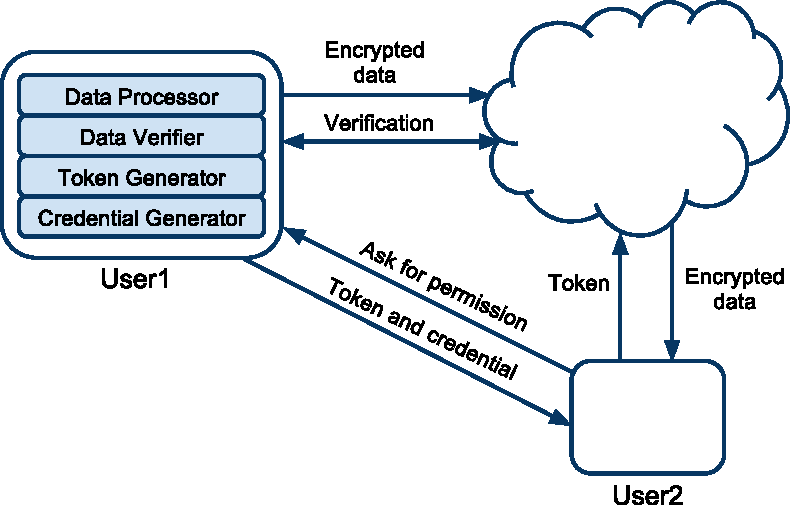
\includegraphics[scale=0.6]{ArchitectureCCSC.pdf}
    \caption{Cryptographic cloud storage, customer scenario.}
    \label{fig:RW:CCS:CA}
\end{figure}

\begin{figure}[h!]
    \centering
    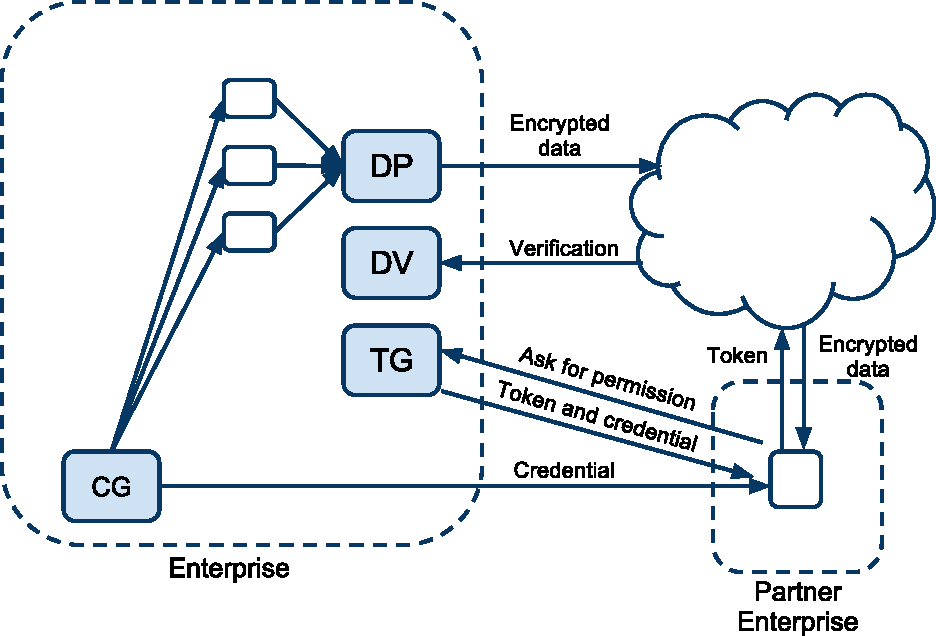
\includegraphics[scale=0.6]{ArchitectureCCSE.pdf}
    \caption{Cryptographic cloud storage, enterprise scenario.}
    \label{fig:RW:CCS:EA}
\end{figure}

The consumer architecture is depicted in Figure \ref{fig:RW:CCS:CA}, and a typical
enterprise architecture is shown in Figure \ref{fig:RW:CCS:EA}.\\

\noindent Each architecture consists of the following computational components:
\begin{description}
  \item[\ac{DP}] \hfill \\Processes data before it is sent to the cloud.
  \item[\ac{DV}] \hfill \\Checks whether data stored in the cloud has been
  tampered with.
  \item[\ac{TG}] \hfill \\Generates tokens that enable the cloud provider to
  retrieve segments of customer data.
  \item[\ac{CG}] \hfill \\Responsible for creating and distributing access
  policies.
\end{description}

The core components are suggested to support \emph{searchable encryption},
\emph{attribute-based encryption} and a \emph{proofs of storage} protocol.

\section{Existing Solutions}
\label{sec:existing}

There are a number of existing solutions for storing data in the cloud,
with more or less of the functionality required to fulfill the problem
description for this thesis. The section highlights some of them.

\subsection{Dropbox}

Dropbox\footnote{\url{http://www.dropbox.com/}} is a popular commercial
application for storing data in the cloud, claiming more than 25 million users
\cite{dropbox_users}. All files are saved using Amazons S3 storage service.

The company boasts strong encryption and strict access control
\cite{dropbox_security}, but has received criticism for its lack of security
\cite{dropbox_concerns}. Among these concerns, is the \emph{Forgotten Password}
feature, which implies that Dropbox can read the users files if they really
want to -- because they have the password -- and that the encryption is
performed server-side.

In addition, Dropbox is not Open Source, and hence one has no way of verifying
that the security features actually work as claimed.

\subsection{Tahoe-LAFS}

Tahoe-\ac{LAFS}\footnote{\url{http://www.tahoe-lafs.org/}} is an open source,
distributed and secure cloud storage file system, which does fulfill
the criteria set in Section \ref{sec:criteria}.
The integrity and confidentiality of the
files are guaranteed by the algorithms used on the client, and is independent
of the storage servers, which may be operated by untrusted people.
This is defined as \emph{provider-independent security} \cite{tahoe}.

In Tahoe-\ac{LAFS}, files are exclusively encrypted client-side, then split up
using \emph{Erasure-coding}, before being uploaded into the cloud\footnote{The
\emph{cloud} in the Tahoe-\ac{LAFS} sense, often refers to other nodes in a so
called \emph{friend net}.}, as illustrated in Figure \ref{fig:B:tahoe}.

\begin{figure}[h!]
    \centering
    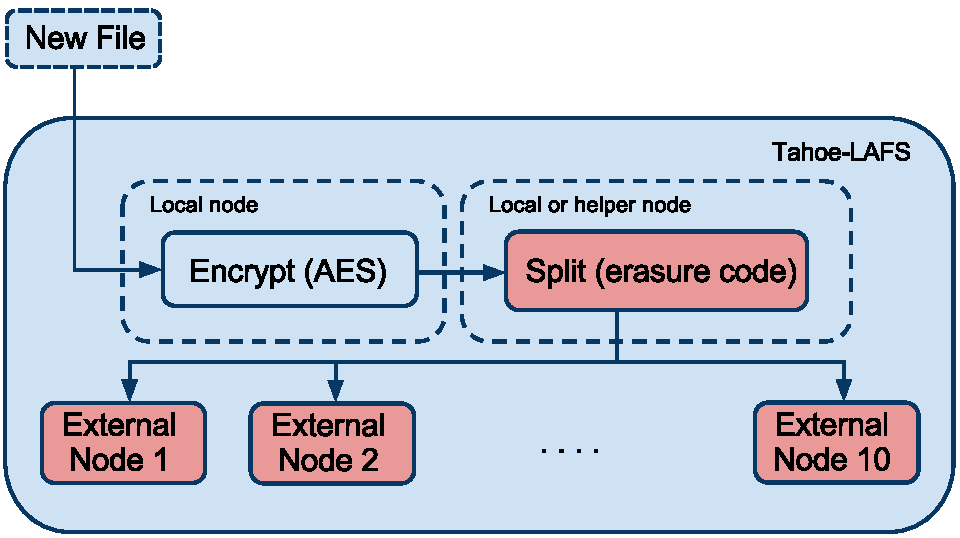
\includegraphics[width=\columnwidth]{Tahoe-newfile.pdf}
    \caption{Tahoe-LAFS: Insertion of a new file}
    \label{fig:B:tahoe}
\end{figure}


\subsubsection{Architecture of Tahoe-LAFS}

Tahoe-\ac{LAFS} has a three layer architecture: the key-value store, the filesystem, and
the application \cite{tahoe}.

The \textbf{key-value store}, is the lowest layer and is implemented by a grid
of Tahoe-LAFS storage servers. Data is kept on the storage servers in the form
of \emph{shares}, which are encrypted and encoded parts of files. Capabilities
are short ASCII strings, containing information on where to find a file, and
how to verify it.  Nodes in the grid learn about each other through an
\emph{introducer}.

The \textbf{filesystem} layer is responsible for mapping human-meaningful
pathnames to pieces of data. Each directory contains a table of capabilities
for its children, i.e. subdirectories or files. Two forms of capabilities is
available for each file, read-only and read-write, and these can be distributed
to e.g. share a file with friends.

Since it is not practical for users to remember strings containing random
characters, the \textbf{application} layer is used for providing a user-friendly
interface to the directories and files.

\paragraph{File Types}

There are two kinds of files in the Tahoe-\ac{LAFS} -- \textbf{immutable} and
\textbf{mutable} files. An immutable file is created exactly once, i.e. it
cannot be modified, and can be read repeatedly. Mutable files can be modified,
and everyone who has access to the signing key can make new versions of
the mutable file. Directories are implemented as mutable files.

\paragraph{Erasure Coding}

Erasure-coding with the Solomon-Reed scheme, enables Tahoe-\ac{LAFS} to recover
a file using only a predefined subset of the parts distributed to the storage
servers. Erasure coding is a type of \ac{FEC} code, which extends a message
with $C$ characters into a longer message with $N$ symbols
\cite{t_reed-solomon}. The original $C$ characters can then be recovered from a
subset of the $N$ symbols.

\subsection{Wuala}

Wuala\footnote{\url{http://www.wuala.com/}} is a closed source secure cloud
storage file system, that seemingly operates very similar to Tahoe-\ac{LAFS}.

The authors have released a paper on a cryptographic tree structure for file
systems, called Cryptree \cite{cryptree}, and has strong focus on reliability
by both providing central servers, in addition to a \emph{P2P cloud} of Wuala
users that has donated capacity to the system.

%**************************************%
\chapter{Technical Procedure}
\label{ch:technical}
%**************************************%

% TODO: Complete this

This chapter will describe a proposed architectural and cryptographic scheme
for providing secure storage of data on a remote untrusted system. It will
further explain the procedures carried out to create a proof of concept
application, that implements the proposed architectural and cryptographic
scheme. The application, named \emph{\ac{CSV}}, is implemented as an
Android application, and consists of a separate server and client functionality.

The chapter will start by giving an overview of the proposed architectural
scheme followed by a more detailed description of the corresponding
cryptographic scheme. The chapter will end by describing the implementation
details for both the server and client side functionality of the Cloud Storage Vault.

\section{Architectural Overview}
%**************************************%
\label{chap:AS}

The architectural solution of a secure cloud file sharing system has to
convince its users that the functions indeed are secure, and that the concepts
are easy to understand and accept. The following sections will elaborate on the
architecture designed by us, favouring simplicity and familiar concepts, such
as files and directories. We also introduce the concept of \emph{capabilities}.

Figure \ref{fig:AS:overview} represents an overview of the functionality that
the architecture must support. The illustration exhibits a user uploading a
file to the cloud, and adding this to a parent directory. After he has done
this, it is possible for him to distribute the capability to other users to
realize sharing of files or directories.

\begin{figure}[h!]
    \centering
    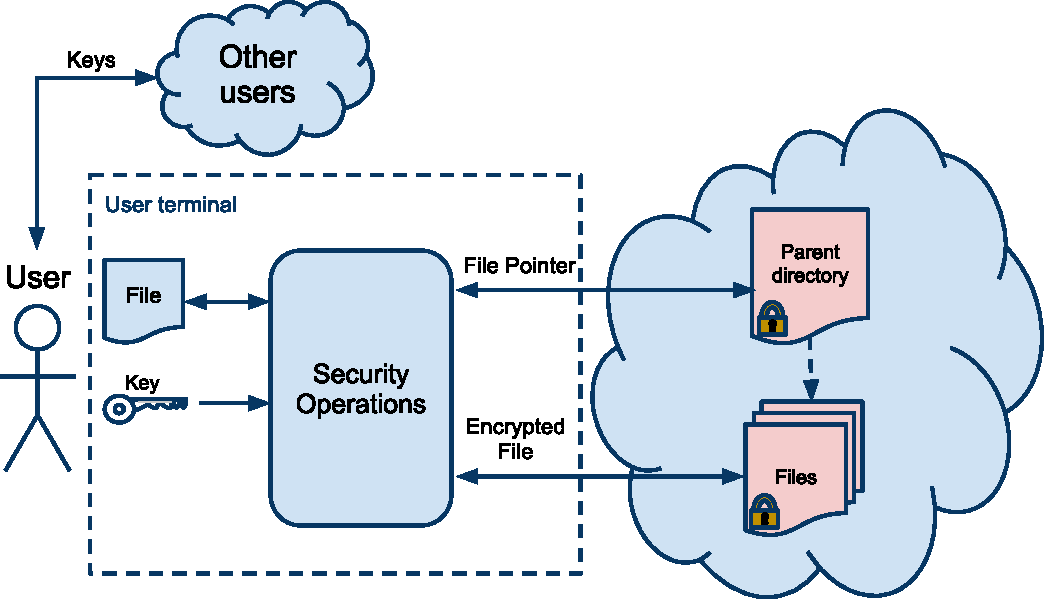
\includegraphics[width=\columnwidth]{ArchitectureOverview.pdf}
    \caption{Overview of user functionality}
    \label{fig:AS:overview}
\end{figure}

\subsection{File Storage}
\label{sec:AS:FS}

The solution for file storage proposed in this thesis, is that only a simple
\emph{key-value store} is needed on the server side. The key works as a lookup
index for a specific value, while the corresponding value equals an encrypted
file object. The server will be required to support the operations of uploading
and downloading key-value pairs to this store.

From the users perspective however, a file object can have multiple forms -- it
can either be a \emph{mutable} or an \emph{immutable} file. A mutable file can
be changed, and is what a user will see as a directory, while an immutable file
is utilized as a normal file.  

A user will need certain information to be able to reach and read a file
object, we define these properties as the \emph{capability} of a file object.
For now, the capability represents the ability to find, read, verify that a
file has not been tampered with, and possibly write to the file object.

\subsubsection{Directory Structure} 

The contents of a directory are files and other directories. More specifically,
a directory contains the means to find files or directories, namely the
capabilities of these file objects. In addition, there exist a human readable
name, an \emph{alias}, for each entry in a directory. This design gives a
flexible and space-conservative structure, since any file object may be found
from multiple directory, but does only exist once in the cloud.

A user will have to have some way of storing the capabilities of his file
objects. This could potentially be done client side, but a problem arises if
the user wants to use several terminals. Thus, we introduce the \emph{root
folder}, a folder from which all other files and folders can be reached. The
user will only need to know of one single capability to reach all his stored
data. This capability needs to be stored and protected by the client in a
password protected \emph{keyring}. The resulting structure is a
directed graph, as illustrated in Figure \ref{fig:AS:filesystem}.

\begin{figure}[h!]
    \centering
    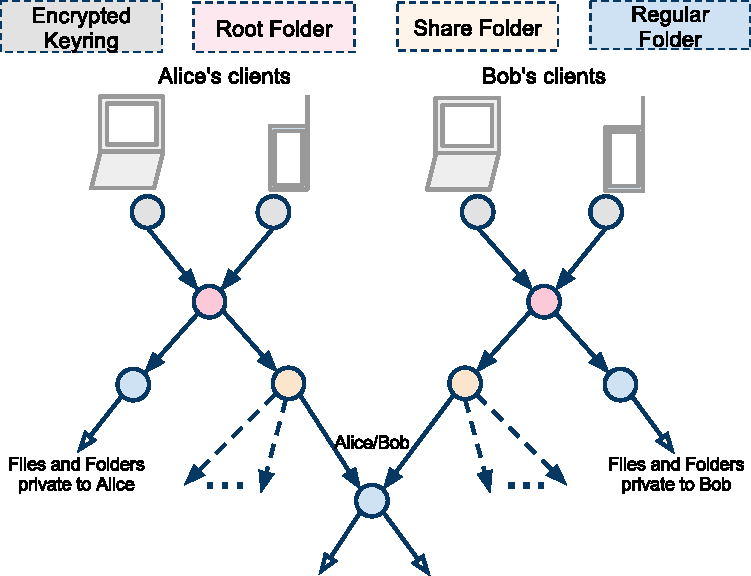
\includegraphics[width=\columnwidth]{ArchitectureFileSystem.pdf}
    \caption{File System Structure}
    \label{fig:AS:filesystem}
\end{figure}

\subsection{ACL/Authentication Layer}

The possession of a capability gives a user access to read a file or read or
write a folder. There are however some properties that the server provider
might want that can not be given by the capability. Therefore a layer
implementing authentication, accountability and possibly more access control
could be preferable.

\subsubsection{Block Access to Encrypted Data}

The capability for a file or folder might be intentionally or unintentionally
leaked by a user. In this case, it would be preferable that the server can
block access to a particular object. The server could also potentially enforce
access rights on all encrypted objects, based on who a user has shared a file
with. This does however require the client to notify the server every time it 
shares a file object with a new person, and is strictly not necessary from a
security standpoint.

\subsubsection{Modification and deletion of objects} 

For each directory, there exist a different capability for read and write
operations, though the read capability can be deduced from the write
capability. From the write capability, it is possible to deduce another secret,
the \emph{write enabler}, which the server also knows of.  Knowledge of the
write enabler is needed for the server to grant access to modify or delete a
folder.

For immutable files, there is no concept of write-access, only read. It is both
illogical and impractical to assume that read access should also yield delete
access. A layer that identifies the creators of a file, can by the same method
decide who should have the rights to delete it.

\subsubsection{Accounting}

If the server side of the system is held by a cloud storage provider, it
is important to be able to decide which users should be billed for the file
\emph{storage} and generated \emph{network traffic}.

In the case of an immutable file, the storage costs can be billed to the user
creating the file. The costs of network traffic can further be charged to the
users retrieving the file.

Accounting might also be interesting for an organization using a third party
cloud provider. For instance an employee who leaves the organization, might be
tempted to copy all the data stored on the server. The organization should then
be able to discover what he has done. 

It is however worth noting that if the accounting happens server side, there is
no real way to verify that all logs stored there are correct, since the cloud
provider will have access to modify or delete them.

\subsection{User Scenarios}

The various user scenarios supported by the software, provides a logical way to
describe the external properties of the system. The fundamental operations are
\emph{downloading}, \emph{uploading} and \emph{sharing} of files.

\subsubsection{Download File}

The download procedure is depicted in Figure \ref{fig:AS:download}. The client
sends a download request with the identifier of a folder, which he possesses
the capability of. The server will respond with the encrypted directory. 
The user will use the capability to decrypt the directory. 

\begin{figure}[h!]
    \centering
    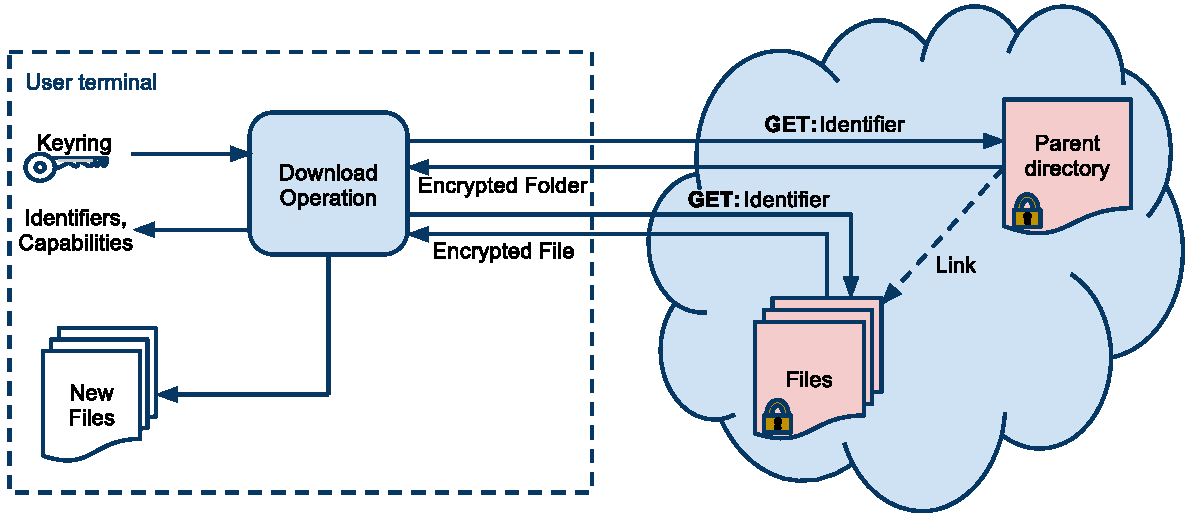
\includegraphics[width=\columnwidth]{ArchitectureDownload.pdf}
    \caption{Scenario: Downloading a file}
    \label{fig:AS:download}
\end{figure}

In the directory, the user finds the aliases and necessary capabilities to gain
access to the children of that folder. If the user now wants to download a file
from the accessed folder, he obtains the identifier for this file through the
capability of the file, and requests the server for this file. Once downloaded,
the capability provides means of decrypting and verifying that the file has not
been tampered with.

\subsubsection{Upload File}

Figure \ref{fig:AS:upload} shows the process of uploading new files. The
capability for the new file is generated by the client, and used to encrypt the
file. The file is then uploaded to the cloud, and the capability and an alias
is linked in to the parent folder of the file. 

\begin{figure}[h!]
    \centering
    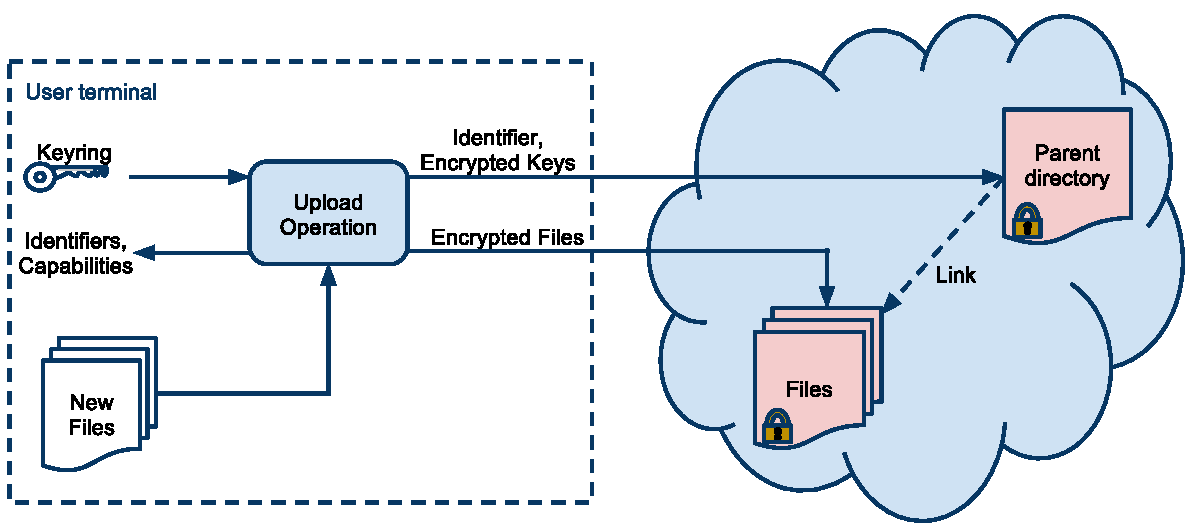
\includegraphics[width=\columnwidth]{ArchitectureUpload.pdf}
    \caption{Scenario: Uploading a file}
    \label{fig:AS:upload}
\end{figure}

\subsubsection{Share Files}

As shown in Figure \ref{fig:AS:sharing}, for Alice to be able to share files
with Bob, she first has to create a new directory that will contain these
files. Alice is then required to share the capability of the new directory with
Bob. When the capability is shared, the new directory will work as a secure
channel where Bob and Alice can share their own folders and files.

\begin{figure}[h!]
    \centering
    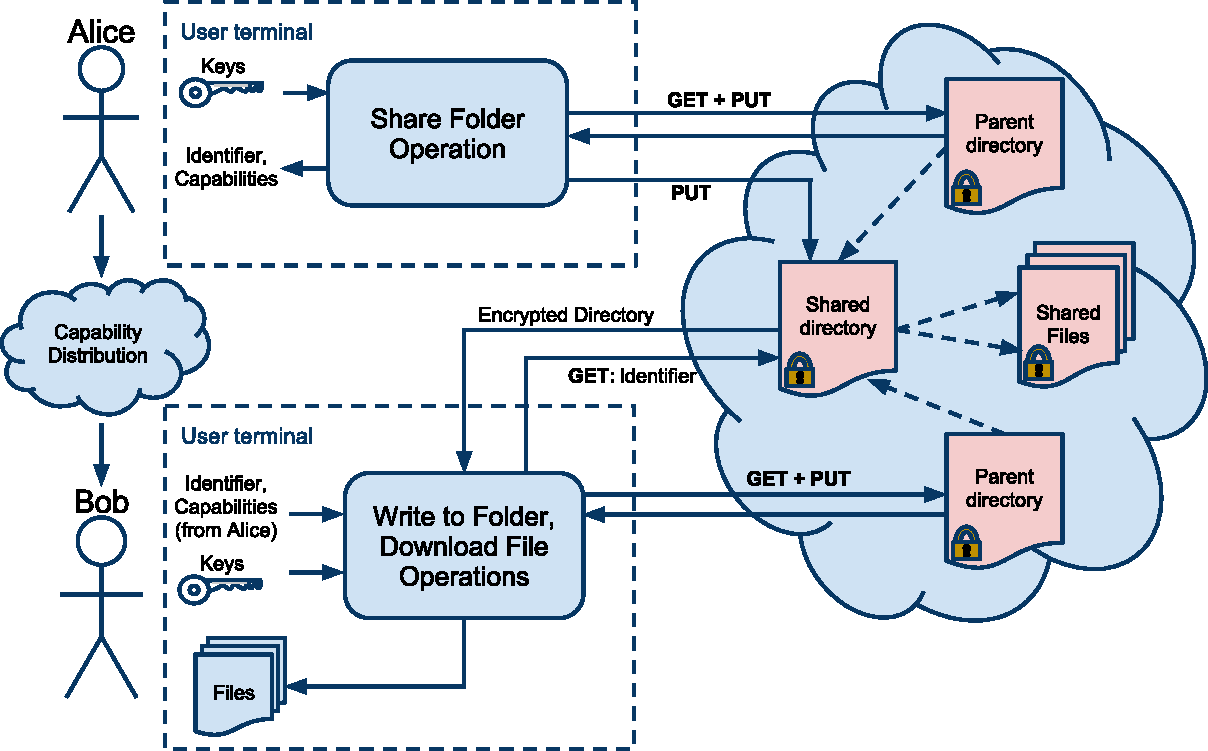
\includegraphics[width=\columnwidth]{ArchitectureShare.pdf}
    \caption{Scenario: Sharing files}
    \label{fig:AS:sharing}
\end{figure}

Before transferring the capabilities to Bob, Alice links the shared directory
to a parent directory, so she can easily find it again at a later time. She can
also link files and other directories to the shared directory.

The capability distribution is a key design issue, and has to be performed in a
secure manner. This can be solved in a variety of ways, and the solutions
proposed in this thesis are discussed in Section \ref{sec:DI:keydist}.

After receiving the capabilities for the shared folder from Alice, Bob requests
and receives the encrypted shared directory, in addition to linking it with a
parent directory for future usage. He can then download shared files as if they
where his own.

\paragraph{Read-Only Shares}

If Alice wants to share a directory in Read-Only mode, she can simply share the
read capability with Bob, instead of the write capability. This will work as
intended, but might prove somewhat cumbersome for Alice. If Alice wants to
write to the directory she has shared with Bob, she can not enter it through
the parent folder shared with Bob, since this will only grant her the read
capability. The implication is that Alice will have to find the directory
another place in her directory tree, to get the write capability.

A more simple solution is to enable Alice to store the write capability
individually among her private files, while storing the read capability in the
shared parent directory. The solution can easily be implemented by using a
specialized \emph{write key folder} under Alice's root folder. The write key
folder will then contain write capabilities to every folder that Alice has
shared in Read-Only mode. The idea behind the write key folder is illustrated
in Figure \ref{fig:AS:readonly}.

\begin{figure}[h!]
    \centering
    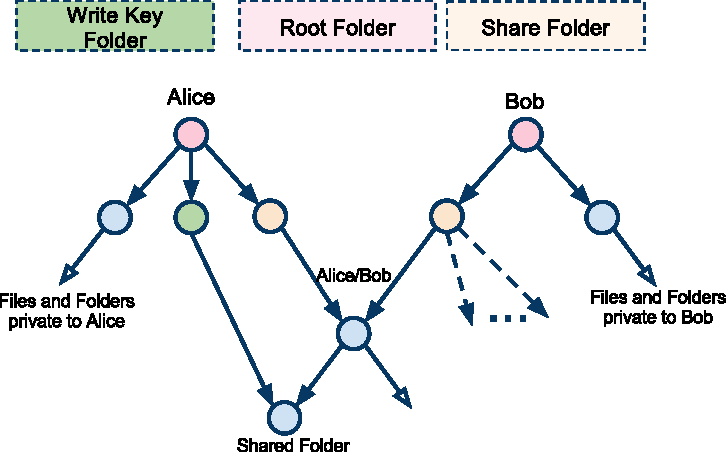
\includegraphics[width=\columnwidth]{ArchitectureShareReadOnlyFolder.pdf}
    \caption{Sharing write-protected folders}
    \label{fig:AS:readonly}
\end{figure}

\subsection{Constraints}

The software using this architecture should be able to run on restricted
devices, i.e. equipment with limited memory and \ac{CPU} power, often in
addition to constraints on power and network utilization.

This has implications for the design of the software, since all cryptographic
operations has to be performed client-side. These considerations will be
brought up throughout the further description of the software.

%**************************************%
\section{Cryptographic Architecture}
%**************************************%
\label{chap:CS} 

This section elaborates on the cryptographic solutions applied to the
architectural scheme in Section \ref{chap:AS}. It will take a closer look at how
confidentiality and integrity can be integrated into the proposed architecture.

%A fundamental scheme for key distribution is needed to realize the desired
%security features, hence an appropriate solution for key distribution will
%also be given.

The section will start with a brief introduction explaining the fundamental security
concepts utilized by the cryptographic architecture. The cryptographic
architecture is further described in terms of file and directory operations. It
is important to mention that some of the cryptographic operations are
taken from key concepts in the TAHOE LAFS \cite{cite}.

\subsection{Security Concepts}

The basic security concept of the application, is to keep the files of a user
confidential to a third-party storage provider. To solve this, the application
encrypts files locally at the user's terminal before uploading them to the
third-party storage provider. 

When accessing a file, the application first downloads the encrypted file
before decrypting it locally. To enable this simple encryption scheme, a user's
terminal is required to locally possess the knowledge of at least one
capability, which contains cryptographic keys to decrypt and verify the
contents of the \emph{root folder}.

The root folder will in turn contain the capabilities for its own children,
which enables the client to decrypt files and folders stored in the root
folder. The other folders work in the same manner.

By initially knowing that files are placed encrypted on a remote server and
that the user possesses one or more cryptographic keys locally, we can continue
with a more comprehensive description of the complete cryptographic solution.
The details are explained in terms of capabilities and the operations conducted
on files and folders.

\subsection{Capabilities}

Capabilities are containers which contain the necessary information to locate,
encrypt, decrypt, verify and possibly write file objects. The contents is
summarized in Table \ref{tbl:capability}. How this information is
created, is somewhat different for files and folders, and is shown in the
subsequent sections. 

\begin{table}
  \centering
  \caption{The structure of a folder entry}
  \begin{tabular}{ | l | l |}
    \hline
    \textbf{Data}       & \textbf{Comment}                          \\ \hline
     Alias              & Human readable name of file/folder        \\ \hline
     Storage Index      & Key to retrive file/folder from server    \\ \hline
     Write Key          & Only for folders, needed to write a file  \\ \hline
     Read Key           &                                           \\ \hline
     Verify Key         & Only for folders, needed to verify a file  \\ \hline
  \end{tabular}
  \label{tbl:folder:contents}
\end{table}


\subsection{Cryptographic Primitives}

The illustrations in the following sections included our chosen cryptographic
primitives. It is however important to note that this cryptographic scheme will
work with other primitives. Any symmetric cipher could work instead of
\ac{AES}, any signing function that uses both a private and public key could be
used, any \ac{MAC} could be used instead of HMAC-\ac{SHA}1, and any
cryptographic hash function could be used instead of \ac{SHA}-256. The security
of the system does however rely on these choices, and the rationale for
each of these can be found in Section \ref{sec:cryptoprimitivechoice}.
%% TODO: Tenk deg litt om

\subsection{File Operations}

This section describes the elementary file operations supported by the
application. The basic operations are \emph{upload file} and \emph{download
file}.

\subsubsection{Upload File} 
\label{sec:CS:CF} 

The operation behind uploading a file, is depicted in Figure \ref{fig:CS:CF}. A
random symmetric encryption key is generated. This is hashed once to obtain the
\emph{storage index} for the file. The storage index is then hashed again to
form the \ac{IV} for the file. 

Next, the file is hashed and the resulting digest is stored together with the
encryption key in the capability. Lastly, the file is encrypted with the
encryption key, and the \ac{IV} is uploaded to the server.

\begin{figure}[h!]
    \centering
    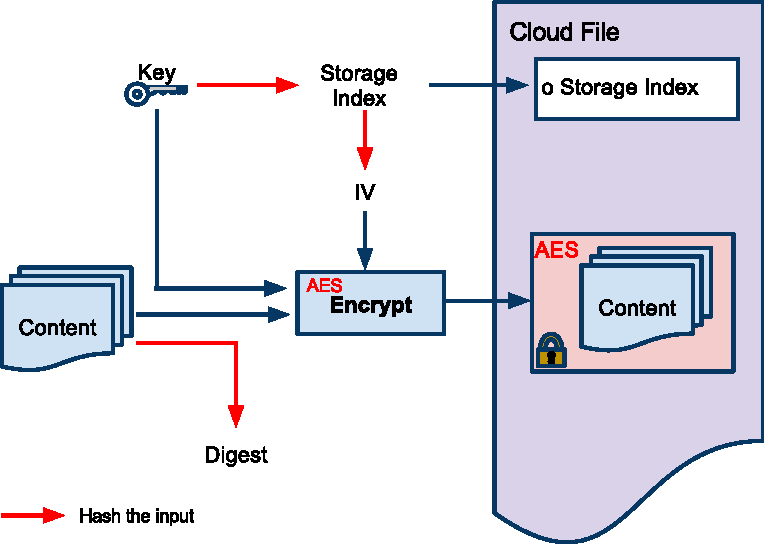
\includegraphics[width=\columnwidth]{CryptoCreateFile.pdf}
    \caption{Uploading a file}
    \label{fig:CS:CF}
\end{figure}

\subsubsection{Download File}
\label{sec:CS:OF}

The process of retrieving a file is illustrated in Figure \ref{fig:CS:OF}. The
storage index is obtained by hashing the stored encryption key extracted from
the capability, and the \ac{IV} is obtained by hashing the storage index. The
file is then downloaded from the server and decrypted. Next, the file is
hashed, and the resulting digest is compared against the digest stored in the
capability. If these two match, the file has not been tampered with.

\begin{figure}[h!]
    \centering
    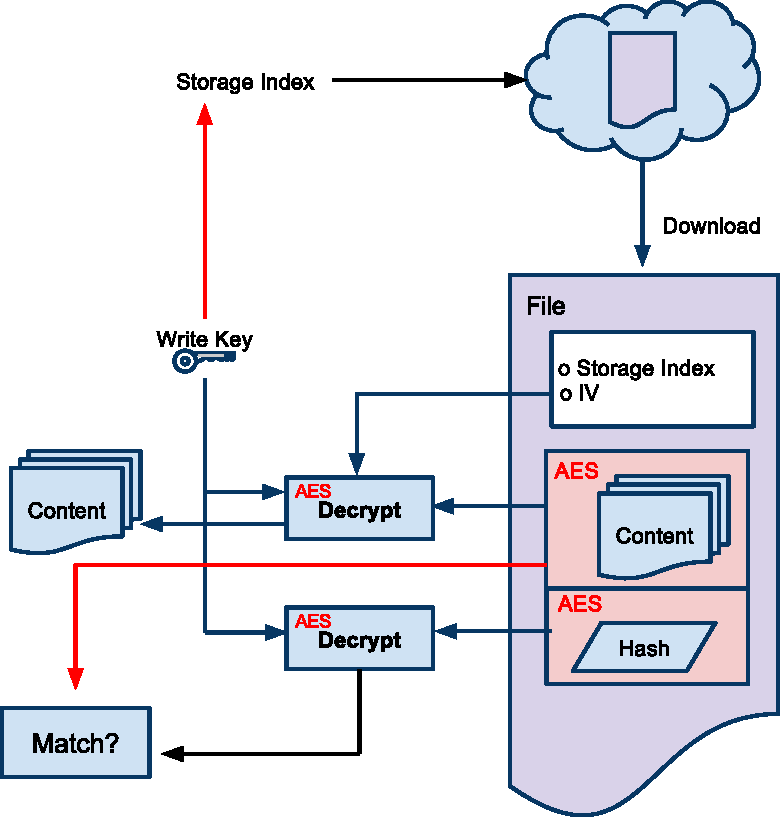
\includegraphics[width=\columnwidth]{CryptoOpenFile.pdf}
    \caption{Downloading a file from the server}
    \label{fig:CS:OF}
\end{figure}

\subsection{Directory Operations}
\label{sec:CS:DO}

This section presents the two basic directory operations used by the
application. The \emph{create directory} and \emph{open directory} operations
are explained as follows.

\subsubsection{Create Directory}

Creating and uploading a directory from the user terminal, is illustrated in
Figure \ref{fig:CS:CD}. The process is a bit more complex than for files,
because it has to support changing the contents of the folder. 

\begin{figure}[h!]
    \centering
        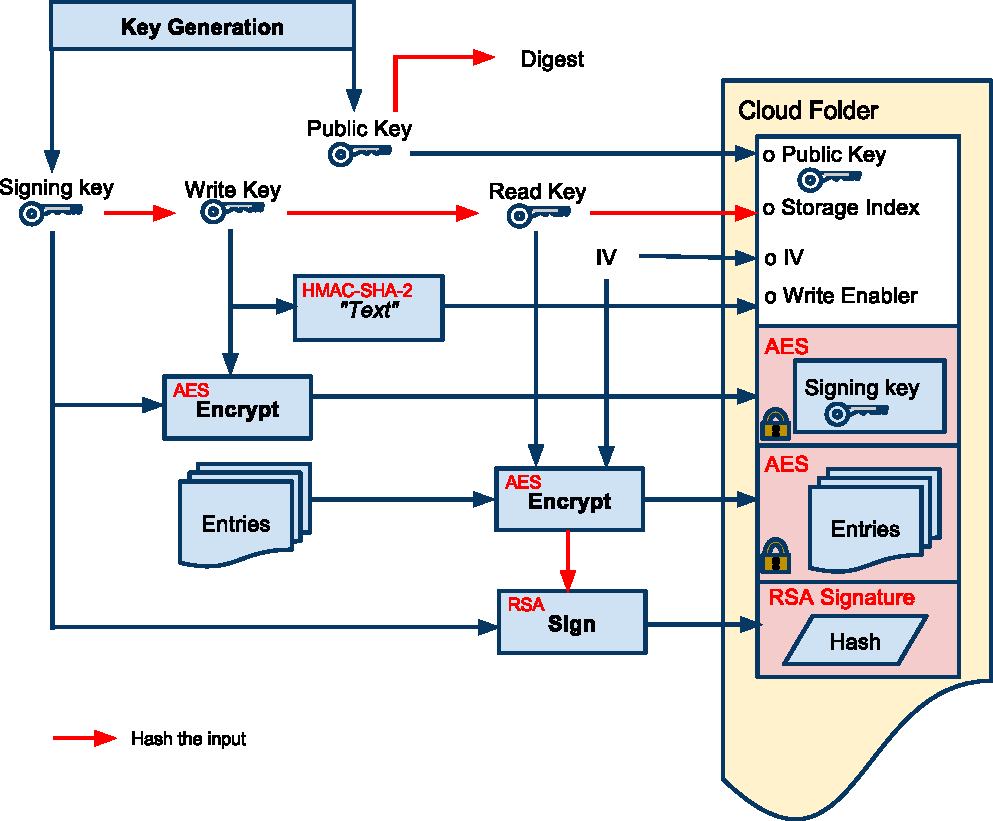
\includegraphics[width=\columnwidth]{CryptoCreateFolder.pdf}
	    \caption{Creating a directory}
    \label{fig:CS:CD}
\end{figure}

Firstly, an asymmetric key pair is generated, and forms the private
\emph{signing key} and the public key. The signing key is hashed to form the
\emph{write key}, and again to form the \emph{read key}, and even once more to
form the \emph{storage index}.

The contents of the folder, which may be empty, is encrypted with the read key
and the resulting ciphertext is signed with the signing key. The signing key is
further encrypted with the read key, and together with the ciphertext, the
public key, the \ac{IV} and the signature, uploaded to the server. 

The \emph{write enabler} is made from the write key with a \ac{MAC} function
and sent alongside the file. The write key is stored together with a hash of
the public key in the capability.

\subsubsection{Open Directory}

Opening a directory involves both downloading, verifying and decrypting the
directory. The verification illustrated in Figure \ref{fig:CS:VOD} and
decryption is illustrated in Figure \ref{fig:CS:OD}. 

\begin{figure}[h!]
    \centering
    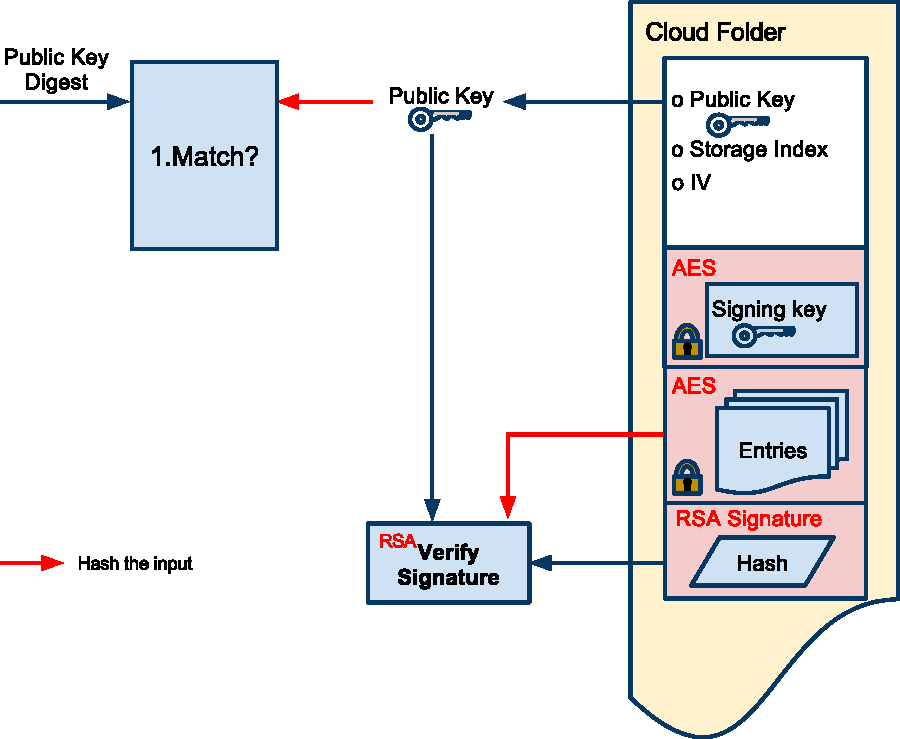
\includegraphics[width=\columnwidth]{CryptoVerifyOpenFolder.pdf}
    \caption{Verifying a directory.}
    \label{fig:CS:VOD}
\end{figure}

\begin{figure}[h!]
    \centering
    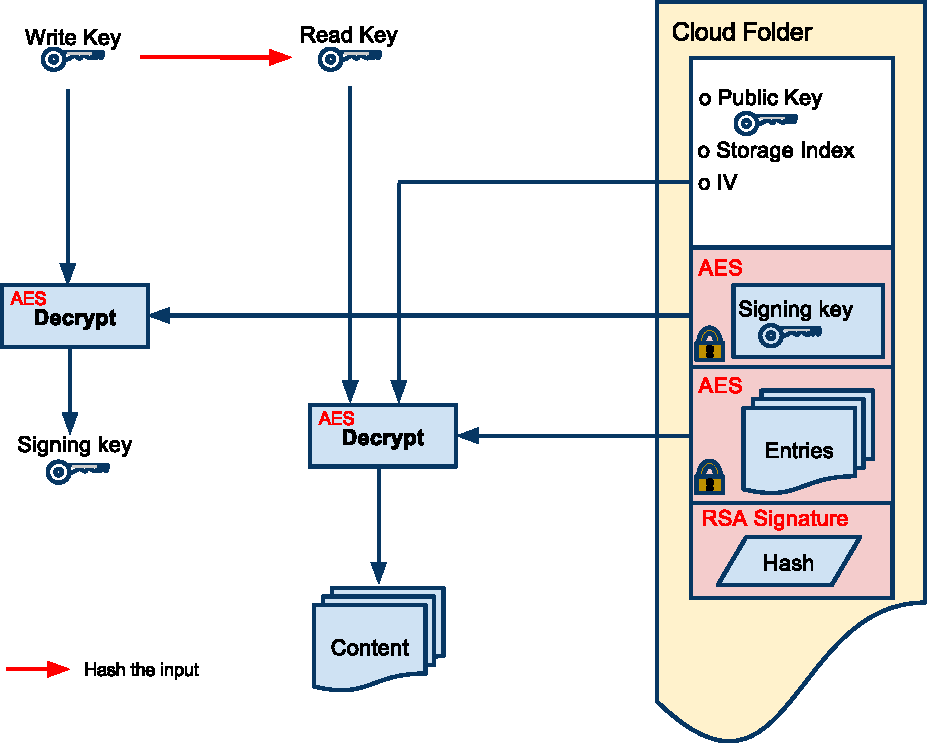
\includegraphics[width=\columnwidth]{CryptoOpenFolder.pdf}
    \caption{Decrypting the contents of a directory and obtaining the signing
    key}
    \label{fig:CS:OD}
\end{figure}

From the capability, the user either obtains the read key or the write key. If
the write key is found, it can be hashed to obtain the read key. The read key
is again hashed to form the storage index, which is used to request content
from the server.

From the server, the user receives the encrypted contents of the folder, the
signature for the folder and the public key. The user verifies that the public
key is correct by hashing it and matching it against a hash stored in the
corresponding capability. Afterwards, the public key is used to verify the
signature. If both these checks pass, the folder is decrypted with the
read key and the content is obtained.

\subsubsection{Modify Directory}

In addition to read the contents of a directory, the user might want to write
to it as well. The process of doing this, is similar to initially creating the
first directory. The key difference, is that the user has the write key in a
capability, and must use this to decrypt the encrypted signing key which he
downloads from the server, instead of generating a new one.
% TODO: Is the sentence above making any sense?

A new \ac{IV} is generated, and the content of the folder is encrypted, and
signed by the signing key. The fresh \ac{IV}, the signature and the encrypted
contents are then uploaded to the server. The write enabler is also sent
alongside, which is deduced in the same way as when creating a new folder.

\subsection{Keychain}

Every user will need to keep a copy of his root capability somewhere.
The capability contains both an encryption key and verification data that a
user will need to safely access his files.

This amount of random data will be hard for a person to remember, and therefore
the capability will have to be stored on the terminal which runs the client
application. Since it might happen that this terminal is either broken in to,
lost or stolen, precautions should be taken to protect the capability on the
device. The normal approach to this, is by using password protection. 

The strength of a password is related to its length and randomness properties.
Passwords shorter than 10 characters are usually considered to be weak
\cite{pbkdf_nist}. In the event of loosing one of the clients, and thus the
encrypted keychain, a potential attacker can use fast password cracking attacks
to try to compromise the root folder keys. As an precaution for this, we will
use \ac{PBKDF2}/RFC2898\footnote{http://tools.ietf.org/html/rfc2898} with a
salt value, to create additional computational work for the process of
unlocking the keychain. This method is known as key stretching
\cite{keystretch}.

\subsection{Choice of Cryptographic Primitives}
\label{sec:cryptoprimitivechoice}

The scheme which has been described in this section requires three primitives;
a cryptographic hash function, a symmetric cipher and an asymmetric cipher
which can be used for digital signatures. The choices should reflect the
following security demands of our application, all with the assumption that the
possible attacker has access to vast quantities of computing power.

% TODO: Sikkerhetskrav bør vi definere tidligere
\begin{enumerate}
    \item It should be infeasible to break confidentiality for any file or folder
    \item It should be infeasible to break integrity for any file or folder
\end{enumerate}

\subsubsection{Symmetric Cipher}
For a symmetric cipher the choice is pretty simple; \ac{AES}. \ac{AES} is
a standard, has been around for a long time, and does not have any serious
security issues as long as it is used correctly.
% Kilder kilder TODO

\section{Server Implementation}

The server, in the most basic form, has to support two operations -- sending
and receiving files. In addition, an \ac{ACL} layer is needed to support user
management and access control to able to allow the deletion of files from the
server.

\subsection{Communication and Architectural Patterns}

By definition, cloud applications are accessible over the Internet. The system
we are creating, should be able to send and receive files and information from
a server in the cloud. The \acf{HTTP} is the foundation of data communication
for the World Wide Web, it is well tested, will pass through most firewalls and
has a multitude of libraries in programming languages. To get a working server
we can also use any existing web server as a foundation, which saves a lot of
work. Thus \ac{HTTP} was chosen as our communication protocol.

\subsubsection{\acs{REST}} The Web is built around an architectural style called
\ac{REST} \cite[ch. 5]{fielding}, which is defined by four interface
constraints: identification of resources, manipulation of resources through
representations, self-descriptive messages, and, hypermedia as the engine of
application state. In addition, \ac{REST} dictates five\footnote{And one
optional, Code on demand, which is not applicable for our system.} architectural
constraints \cite{fielding}. Our server application adheres to these
constraints or \emph{patterns} as follows:

\begin{description}
  \item[Client-server] \hfill \\
    The server is our server application, and the client is the various client
    applications,

  \item[Stateless] \hfill \\
    Since the server is just a simple key-value file store, it does
    not need to keep state.

  \item[Cacheable] \hfill \\
    The server could easily add caching, by putting each encrypted file in
    memory as downloaded, and using the Least-Frequently Used algorithm for
    choosing which items to swap out. In addition, for every update of a folder,
    the corresponding cache item has to be marked as invalid.

  \item[Layered system] \hfill \\
    Layers are used to encapsulate, separate and hide functionality.
    Figure \ref{fig:IM:layers} illustrates the layers of the server application.

  \item[Uniform interface] \hfill \\
    The interface between clients and server(s) are given by the URI scheme in
    Table \ref{tbl:IM:restinterface}. When a folder is uploaded a Write Enabler
    must also be provided together with the storage index..
\end{description}

\begin{figure}[h!]
    \centering
    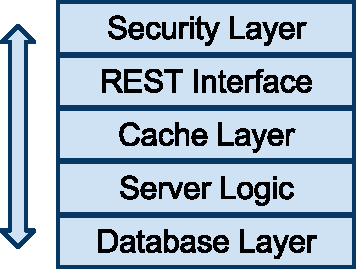
\includegraphics[scale=0.6]{ImplementationServerLayers.pdf}
    \caption{Architectural Layers in the Server application.}
    \label{fig:IM:layers}
\end{figure}

\begin{table}[h!]
    \centering
    \caption{The \acs{REST} interface of the server application.}
    \begin{tabular}{|l|l|}
        \hline
        \multicolumn{1}{|c}{\textbf{\acs{URI}}} & \multicolumn{1}{|c|}{\textbf{Description}} \\
        \hline
        \texttt{/put/<storage index>} & Creates or updates encrypted file \\
        \hline
        \texttt{/get/<storage index>} & Retrieves encrypted file \\
        \hline
    \end{tabular}
    \label{tbl:IM:restinterface}
\end{table}

In this context, resources are the encrypted files, and the architectural
constraints of \ac{REST} also matches that of our system as a
whole. Thus, the server application are designed in a \acs{REST}ful manner.

\subsubsection{Network Security} Since we are utilizing \ac{HTTP}, we can
easily add an extra layer of \ac{TLS} to form \ac{HTTPS}. This makes it more
difficult for potential attackers to intercept messages, and also provides
protection against the most basic form of \ac{MITM} attacks. It also provides
protection against eavesdropping, which would have revealed the Write Enabler
for folders and could be used by an attacker to delete user files. The top-most
layer of Figure \ref{fig:IM:layers} thus refers to \ac{TLS}.

\subsection{Environment}

The Python programming language in a Linux environment was chosen as development
platform, together with a set of applications, interfaces and micro frameworks.
The rationale for each of these follows.

\paragraph{Python} Python is a high-level general-purpose programming language.
It was chosen due to previous knowledge and experience by the
authors, in addition to its simplicity.

\paragraph{Apache} The Apache HTTP Server is a well tested and used web
server. According to \citet{netcraft}, Apache is by far the most used web server
software, and has been so since 1996. It was chosen on the basis of previous
experience and its superb documentation.

\paragraph{\acs{WSGI}} The Python \ac{WSGI} is, as the name suggests, an
interface between a web server and a Python application. It is defined in
\ac{PEP} 3333\footnote{\url{http://www.python.org/dev/peps/pep-3333/}}, and
specifies both sides of the interface -- the \emph{application} and the
\emph{server}. The server side is implemented in the form of an Apache
module, namely \texttt{mod\_wsgi}, and the application is where we put our
code.

For each of the requests the server (i.e. \texttt{mod\_wsgi}) receives, a call
to the application function is made with two arguments -- a data structure
containing the environment variables, and a callback function for which the
application uses to return data to the requesting user via the server.

\paragraph{Pyroutes} To adhere to the \ac{DRY} principles, we chose to make use
of a micro framework around \ac{WSGI} called
Pyroutes\footnote{\url{http://www.pyroutes.com/}}. It provides shortcuts for the
most frequently used functionality when developing web services, as that of
\ac{URL} handling and processing of submitted user data in the form of
\texttt{GET} and \texttt{POST} requests.

Pyroutes did not, however, support the HTTP \texttt{PUT} request, so this was
implemented and contributed back to the project.

\subsection{Implementation Details}

The code was structured as illustrated in Figure \ref{fig:IM:layout}. The file
\texttt{handler.py} provides the interface for \texttt{mod\_wsgi} and the server
application, and basically includes the \ac{URL} scheme in
\texttt{fileserver.py}. An example \ac{URL} mapping is shown in Listing
\ref{lst:IM:get}. The function \texttt{get\_file} is registered to have the
\ac{URL} \texttt{/get} through the decorator provided by Pyroutes. After
retrieving the file from disk, a proper \ac{HTTP} response is returned,
containing required headers.

The file \texttt{filesystem.py} contains the low-level file system operations,
\texttt{save\_file()} and \texttt{retrieve\_file()}, together with a set of
helper functions to manage file access checking and database operations.  The
folder \texttt{sql/} contains \ac{SQL} code to create necessary tables in the
database, and \texttt{db.py} provides an helper function to connect to the
database.

\begin{figure}[h!]
\begin{verbatim}
|-- cloudstorage
|   |-- __init__.py
|   |-- db.py
|   |-- fileserver.py
|   |-- filesystem.py
|   |-- settings.py
|   `-- sql
|       `-- write_enablers.sql
|-- handler.py
`-- tests
    `-- filesystem_tests.py
\end{verbatim}
    \caption{Server module structure}
    \label{fig:IM:layout}
\end{figure}

\lstinputlisting[language=Python,breaklines=false,label=lst:IM:get, caption=URL mapping in fileserver.py]
{listings/fileserver.py}

\subsubsection{\acs{ACL} functionality}

The only \ac{ACL} functionality implemented, is the server-side verification
that a client has proper access to overwrite a file, e.g. when a client wishes
to update a folder with new contents. We call this \textbf{Write-Enabler
Verification}.

When a client first uploads a new folder, it also provides a
\emph{Write-Enabler Key}, which the server adds to the database along with the
\emph{Storage Index} of the folder.  For every subsequent request to write to a
file with this specific Storage Index, the server verifies that the provided
Write-Enabler Key is equal to that in the database.

If a client tries to put a file with a Storage Index that already exists, the
server replies with an error code if the client in addition does not provide a
valid Write-Enabler Key.

\section{Client Implementation - Android}

The \ac{PoC} client we have implemented, is made for devices using the Android
operating system, which is based on Linux. The \ac{SDK} for making Android
applications, is essentially a somewhat modified version of Java.

Most devices that use the Android operating system are mobile phones or
tablets, which implies that they are limited in terms of speed and
memory. The point of making the \ac{PoC} client for such a device, i.e. a
\emph{smart phone}, is the growing availability, and the flexibility these
devices provide. A user carries the device everywhere, it has a network
connections, and it is always on.

A nice side effect of developing on a smart phone platform, is that if the
software performs well on a constrained device, it will almost certainly also
have good performance on any faster device as well.

\subsection{Environment}

The \ac{PoC} client was made on the Android platform and written in the Java
programming language, together with a set of frameworks. The rationale for
these are as follows.

\paragraph{Android} The Android operating system is made by Google, and is most
commonly found on mobile phones and tablets. The platform choice of Android was
done based on hardware availability and familiarity with developing on the
platform and the programming language (Java).

\paragraph{Java} Java is a high-level, object-oriented programming language.
Applications written in Java runs in a \ac{JVM}, which implies that a Java
application can run on almost any device which has a \ac{JVM}.

The ``\ac{JVM}'' on Android is called \emph{Dalvik}, but it is strictly not a
\acl{JVM} as the bytecode on which it operates is not Java bytecode.
After the regular Java compiler has created the \texttt{.class} files, a Dalvik
tool transforms them to another class file format called \texttt{.dex}
\cite{dalvik}.

\paragraph{HttpComponents} Apache HttpComponents are a set of libraries for
\ac{HTTP} transport in Java. The part used in our client is called HttpClient.
Android incorporates parts of this client in its runtime environment. The use
of this library adheres to the \ac{DRY} principles.

\paragraph{\ac{JCA}} \ac{JCA} is an architecture for doing cryptographic
operations in Java. The architecture is based on principles of implementation
independence, implementation interoperability and algorithm extensibility.
Basically what this means, is that each implementation of the \ac{JVM} can have
different implementations of the cryptographic primitives, but the developer
does not need to know which implementation is available.

\paragraph{ZXing Barcode Scanner} ZXing Barcode Scanner is a popular Android
application which can be used by other Android applications to both scan and
generate barcodes. By the use of this application, we adhere to the \ac{DRY}
principles, by not creating our own code to generate barcodes.

\subsection{Architectural Patterns}

\paragraph{Client-Server} It should be obvious that the client we have
implemented is the client part of the overall client-server pattern.

\paragraph{Pipe-and-Filter} The basis of the pipe-and-filter pattern is that
there exist a chain of processing elements, where the output of one element is
the input of the next element. We use this for file uploads and downloads to
limit the memory usage of the client, as well as to increase performance.

\paragraph{Asynchronous Pattern} We use asynchronous calls to slow operations
-- e.g. file upload and key generation -- extensively, to prevent the interface
from hanging and to deliver a smoother user experience in general.

\subsection{Implementation Details}

\subsubsection{Structure}
% Package Structure, some nice UML (?)
% Which qualities do we wish to achive? Security, Performance, Usability

The source of our client is logically separated into two entities --
\textbf{CSVlib} and \textbf{CSVAndroid}. CSVlib is a pure Java library which
contain the necessary entities, cryptographic operations and communication
calls required for the client. CSVAndroid contains primarily a graphical user
interface to make use of CSVlib on an Android device.

\subsubsection{Cryptographic Entities}
All the cryptographic entities -- namely folders, files and capabilities -- are all
part of CSVlib. Their relationship can be seen in Figure \ref{fig:CSVlib:overview}.

\begin{figure}[h!]
    \centering
    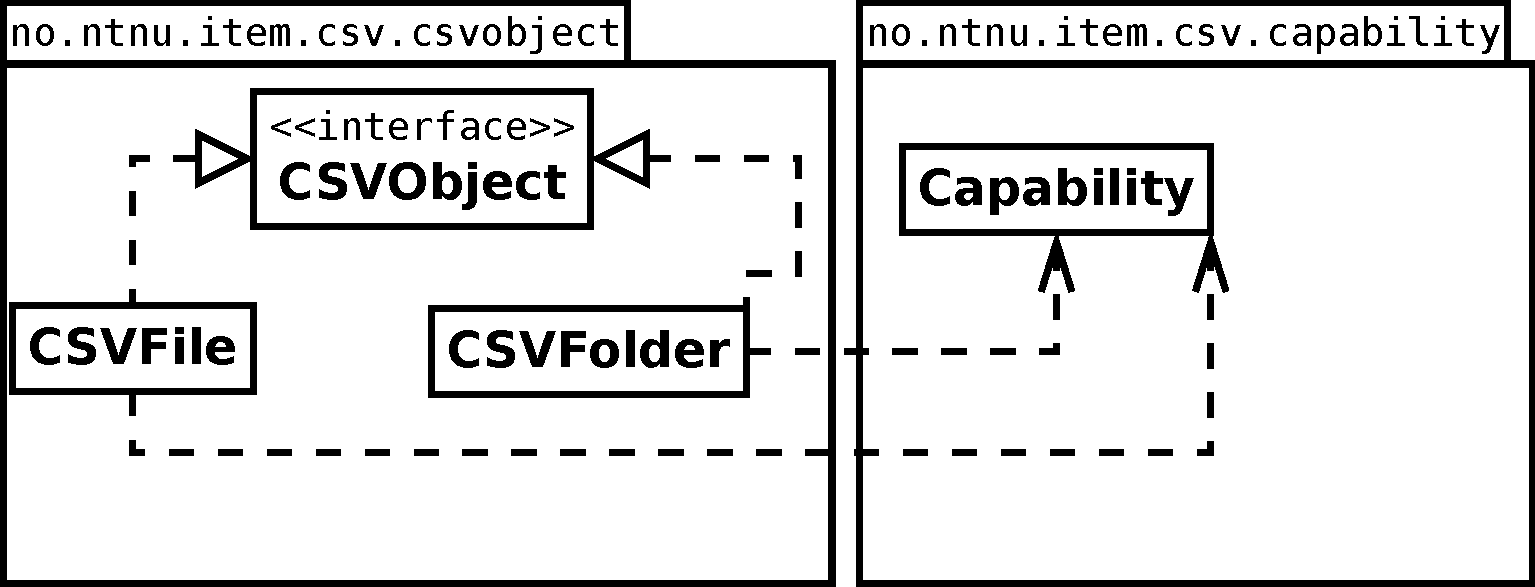
\includegraphics[scale=0.4]{csvobjects.pdf}
    \caption{Cryptographic entities and their relations}
    \label{fig:CSVlib:overview}
\end{figure}

\paragraph{Capabilities} Capabilities are containers for
cryptographic keys and information to identify a corresponding object. A
capability will contain information to identify an object as either a file or a
folder, and have the information to read, write or verify that object.

Capabilities are stored server side in folders, in it's serialized form shown
in Figure \ref{fig:CAP:serial}. \emph{Object Type} specifies if the capability
represents a file or a folder, with values \emph{F} or \emph{D}
respectively.

\begin{figure}[h!]
    \centering
    
\includegraphics[scale=0.6]{CapabilitySerialization.pdf}
    \caption{Serialized form of a capability}
    \label{fig:CAP:serial}
\end{figure}

\emph{Key Type} specifies the permissions the key will grant on the object and
can be either \emph{RO} (Read Only), \emph{RW} (Read and write) or \emph{V}
(Verify).

The different parts are separated by the character \textbf{:}. The key and
verify string are encoded in Base32, which means that the 128 bits these
strings are represented by, will be replaced by an alphabet of 32 different
symbols, namely A-Z and 2-7. This transformation will give some overhead in
storage and transfer (26 bytes compared to 16), but makes it possible to read for a human
with few mistakes or misunderstandings.

\paragraph{Folders}

A folder is represented by the class \textbf{CSVFolder}. A CSVFolder object is
a collection of aliases and their corresponding capabilities. For
the most part, the data stored in a folder is so small that it can easily live for
as long as needed in the memory of the client.

When a folder is created or updated, the content is serialized and encrypted,
before it is uploaded to the server directly from memory. The serialization for
each item in a folder is simply \textbf{alias;capability}, where the capability
itself is also serialized.

\paragraph{Files}

A file is represented by the class \textbf{CSVFile}. While a folder in general is small,
a file can be of any size, even larger than the space the \ac{RAM} on the
device itself represents.

To keep the memory footprint low, we use the pipe-and-filter architectural
pattern to stream data all the way from the cloud to the disk, or vice versa,
through encryption and verification.

An example of how we do this for uploads is shown in Listing
\ref{lst:inputstream}.

\lstinputlisting[label=lst:inputstream, caption=Pipe and filter upload of a file]
{listings/fileupload_example.java}

The \emph{InputStreams} are chained together, with the effect that a read from
\emph{readBuffer} will trigger a read trough the whole pipe. The
\emph{DigestInputStream} will update the state of the hash function, but is
transparent in the sense that whatever goes into the stream will also be what
comes out. The \emph{CipherInputStream} on the other hand, will output an encrypted
stream of the data from the file. Buffers are placed between each step of the
stream for some performance increase.

\subsubsection{Communication with Server}
% Do not repeat what is said in Server equivalent section
% Apache commons, Serialization of objects

For \ac{HTTP} transport we utilize the Apache Software Foundations
HttpComponents Client\footnote{ \url http://hc.apache.org/} also known as
HttpClient.

This Client offers support for authenticated requests to a server, and both
upload and download through \textbf{PUT} and \textbf{GET} requests respectively.
We wrap communication with the server in two classes,
\texttt{Communication.java} and \texttt{CSVFileManager.java}.
\texttt{Communication.java} provides functionality for sending and retrieving
data from our server, while \texttt{CSVFileManager.java} provides specific
methods for sending and receiving the encrypted objects, CSVFile and CSVFolder.

\subsection{Sharing}
% Sequence Diagram - How we use the cryptographic solutions (and which ones) to
% achieve sharing, securely

A \emph{shared folder} is basically just a folder object which two or more
people have the required encryption keys for.

The problem of creating a share with someone, is that you have to verify that
you are actually sharing with the correct person. The data, or \emph{secret},
that will have to be shared, is a serialized form of the capability of the
shared folder, as shown in Figure \ref{fig:CAP:serial}.

The client supports two methods of doing this. The most cumbersome
is having to manually copying the key from one users client to another, and
afterwards verifying that the key for the selected folder is correct. An example
of this can be seen in Figure \ref{fig:CSVAndroid:manualimport}. This feature
is also needed to support out-of-band methods for establishing a share.

\begin{figure}[h!]
    \centering
    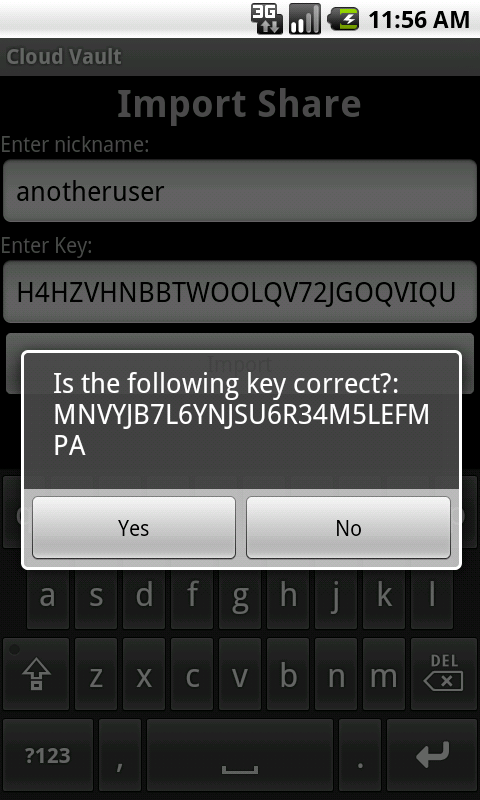
\includegraphics[scale=0.4]{client-manualimport.png}
    \caption{Establishing a share by copying the key}
    \label{fig:CSVAndroid:manualimport}
\end{figure}

The other possibility is to make use of a \ac{QR} code, which is a matrix
barcode that can store information. What this means is that one user will
generate a barcode on his device, and the other user can scan that code using
the camera on his device. Figure \ref{fig:CSVAndroid:barcode} illustrates how
this code will look. The barcode contains both the key and the verification for
the shared folder. Once two users have shared a folder once, that folder can be
used for all future shares, which means that the two people will never have to
meet and do the capability exchange again. The identity has thus been verified.

\begin{figure}[h!]
    \centering
    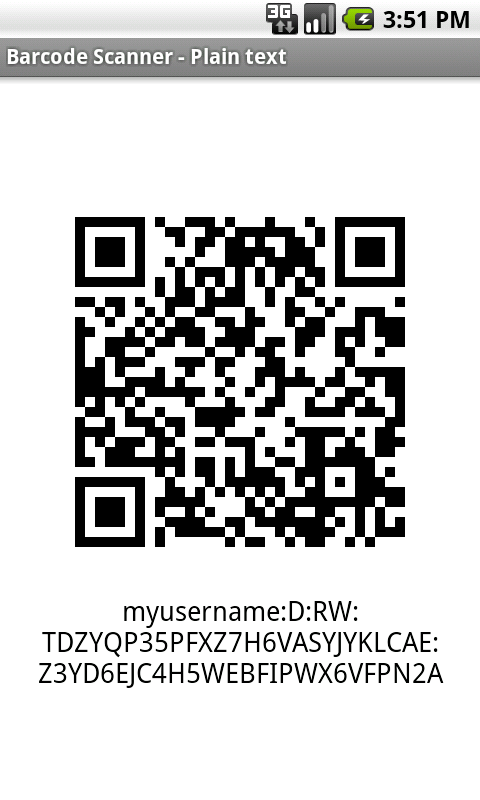
\includegraphics[scale=0.4]{client-barcode.png}
    \caption{Establishing a share by using barcodes}
    \label{fig:csvandroid:barcode}
\end{figure}

\subsection{Adding a New Client}

Using more clients, or different devices, is almost the exact same as sharing,
and is solved in the same manner. The only difference is that the capability
that needs to be transfered, is that of the \emph{root folder}. It is also
possible to take any other folder and use as a new root for the new client if
that is the users wish.

\subsection{Securing the Client}

For a user to access his root folder, the client will have to know the
capability of that folder. This is clearly to much for a user to remember, so
the capability will have to be stored on the client. However, the client might
be stolen or broken into by some means, and if the capability is stored in clear
text, it is easily stolen.

We partially remedy this by the use of the \ac{PBKDF2} algorithm, which makes an
encryption key from a password. This generated key is used to encrypt the root
capability in a file stored on the client. We call this the encrypted key ring.

These precautions are however no defense if the attacker managed to read the
memory while the key is unlocked. The client enforces that this password should
be at least 9 characters long.

\subsection{User Interface}
% goal: As easy as possible!
% First start: Generate new cap/import an old one (Adding a new client section)
% Browsing remote file(s)/folders
% Sharing a file - first/following times - Key Distribution
% Uploading/Downloading file

We have tried to make a user interface that is easily understandable by a novice
user, both in terms of \emph{where to click} and in terms of how we name
cryptographic operations. For instance we never use the word \emph{capability}
in the client.

\paragraph{Main Screen}

The main screen of the application is shown in Figure
\ref{fig:CSVAndroid:mainscreen}. However, before the user gets to this screen,
he will have to unlock his local keyring with his password. If it is the first
time the user starts the application, he will have to enter his online
credentials, and gets a choice to either import an existing root folder, or to
generate a new one. In both cases the user will have to choose a password to
encrypt the root capability in to the local keyring.. From the main screen the
most common action would be to \emph{Browse the vault} -- in other words to see
the files that the user has stored in the cloud.

\begin{figure}[h!]
    \centering
    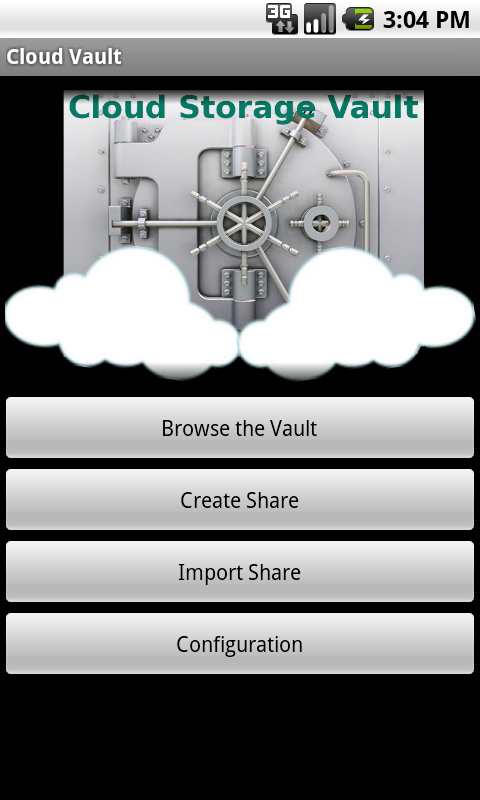
\includegraphics[scale=0.4]{client-mainscreen.png}
    \caption{Main screen of client}
    \label{fig:CSVAndroid:mainscreen}
\end{figure}

\paragraph{Browse the Cloud}

The interface for browsing the files stored in the cloud is made in what we
understand as a common and understandable way of interpreting users actions on
the android platform, and can be seen in Figure
\ref{fig:CSVAndroid:remotebrowse}. Tapping a file will download that file, and
tapping a folder will open that folder.

\begin{figure}[h!]
    \centering
    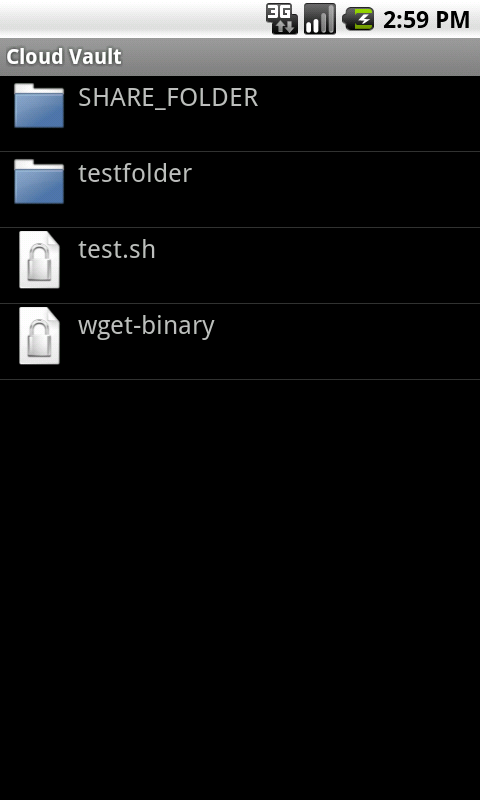
\includegraphics[scale=0.4]{client-remotebrowse.png}
    \caption{Browsing the cloud storage from client}
    \label{fig:CSVAndroid:remotebrowse}
\end{figure}

An upload is treated in a similar way. To reveal this option, the user have to
press the \textbf{Menu}-button. The user will then be allowed to browse his
local filesystem for the file he wishes to upload, and tapping that file will
start the upload.

A long press on a file, or a folder item, will reveal the context menu shown in
Figure \ref{fig:CSVAndroid:remotecontext}. The least understandable action is
probably \emph{Unlink}, which remove a file or a folder from the parent folder.
The reason why it says unlink and not delete, is that a file can potentially be
linked in a number of different folders, and it is impossible by our design to
reveal which folders the file has been linked to, except the one that we are
unlinking from.

\begin{figure}[h!]
    \centering
    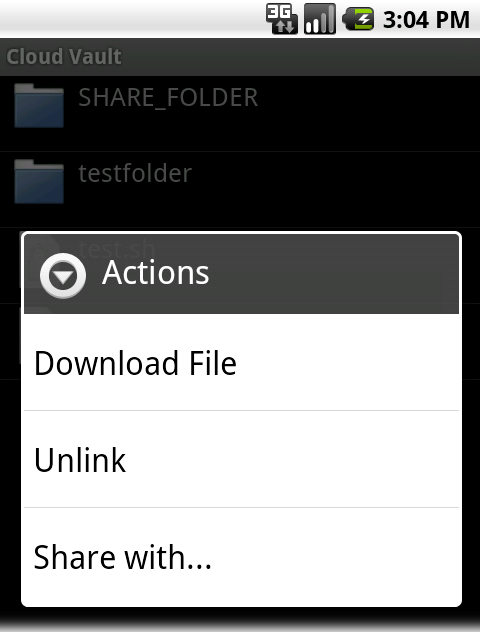
\includegraphics[scale=0.4]{client-browsecontext.png}
    \caption{Context menu}
    \label{fig:CSVAndroid:remotecontext}
\end{figure}

%**************************************%
\chapter{Experimental Procedure}
\label{ch:experimental}
%**************************************%

This chapter will explain the experimental procedures performed on the Cloud
Storage Vault. It will start by explaining the measurements on the performance
of the application. The performance is further compared to similar existing
network applications. Finally, the chapter will go through the experimental
procedures of measuring some aspects of the security of the system.

\section{Performance}

We have tested the client part of the application on two Android phones, an HTC
Desire and an HTC Hero. We have also tested the Java libraries on a
desktop computer. The specifications for HTC Desire can be seen in Table
\ref{tbl:device:desire}, for HTC Hero in Table \ref{tbl:device:hero}, and the
desktop computer in Table \ref{tbl:device:computer}.

\begin{table}
  \centering
  \caption{HTC Desire Specifications}
  \begin{tabular}{ | l | l |}
    \hline
    Name    & HTC Desire                        \\ \hline
    CPU     & Qualcomm Snapdragon QSD8250, 1 GHz \\ \hline
    Memory  & 576 MB \ac{RAM}                   \\ \hline
    Storage & Samsung Micro SDHC Class 2, 4 GB  \\ \hline
    System  & Android 2.2, Linux 2.6.32.15      \\ \hline
  \end{tabular}
  \label{tbl:device:desire}
\end{table}

\begin{table}
  \centering
  \caption{HTC Hero Specifications}
  \begin{tabular}{ | l | l |}
    \hline
    Name    & HTC Hero                          \\ \hline
    CPU     & Qualcomm MSM7200A, 528 MHz        \\ \hline
    Memory  & 288 MB \ac{RAM}                   \\ \hline
    Storage & Micro SDHC Class 6, 4 GB          \\ \hline
    \ac{OS} & Android 2.2, Linux 2.6.29.6      \\ \hline
  \end{tabular}
  \label{tbl:device:hero}
\end{table}

\begin{table}[!h]
    \centering
    \caption{Test computer Specifications}
    \label{tab:hwbf}
    \begin{tabular}{| l | l |}
	\hline
	Product		        &HP Compaq 8100 Elite SFF PC \\
	\hline
	CPU		            &Intel(R) Core(TM) i7 CPU 860 @ 2.80GHz\\
	\hline
	Memory	            &4GB \ac{RAM}\\
	\hline
    Storage             &Hitachi HDS72105 SATA2 \\
	\hline
    OS		            &Ubuntu 10.10 64 bit\\
	\hline
	Kernel Version	    &Linux 2.6.35\\
	\hline
    Network             &1Gbit wired Ethernet \\
    \hline
    \end{tabular}
\end{table}


\subsection{Eliminating Bottlenecks on Android Devices}

On the Android devices, we identify three possible bottlenecks that we might be
able to control: The \emph{network}, our \emph{application} by itself and the
\emph{memory card}.

The mobile phones will normally obtain their network connection through a
wireless protocol that varies naturally in throughput, e.g. \ac{UMTS}. While
these protocols work just fine, from a measurement standpoint, we want to have
a fast and stable connection. Our solution was therefore to connect the Android
devices to the test computer, and use the computers network through the
\ac{USB} interface.

Another bottleneck, might be the memory card. The \emph{class} of a memory card
will identify the least sustained write speeds obtainable from the card in a
fragmented state \cite{sdcard}. The class number $X$ represents this guarantee
in $X$ MB, so a Class 2 card guarantees a speed of 2 MB/s. However, there are
the possibility that the card can perform significantly better than what the
class number indicates.

\subsection{What is Measured}

For \emph{files}, we measure the bandwidth the client uses when uploading and
downloading a file. This is accomplished by measuring the network traffic on
the server, and record this. For comparison, we also deactivated hashing and
encryption in the processing pipeline on the client, and recorded the network
traffic.

\emph{Folders} are relatively small in size, so the network should not be a
bottleneck. However, the different cryptographic operations might take some
time, as will the serialization of folders. The following were measured for
folders:

\begin{enumerate}
    \item The average time it takes to create a folder
    \item The time it takes to encrypt and sign a folder, with varying amount
        of data
    \item The time it takes to verify a newly downloaded folder, with varying
        amount of data
    \item The time it takes to serialize a folder, with varying amount of data
\end{enumerate}

\subsection{Sources of Error}

The trouble with measuring performance on operations that are relatively quick,
is that they are very vulnerable to \emph{noise} from the system. The Android
system comes with a lot of built-in services that runs sporadically, and hence
affect the measurements. However, the small and quick operations are not
necessarily facinating to measure -- the interesting behaviour to observe is
how their performance is affected when the amount of data is increased. The
goal of the client is to deliver a quick and smooth experience for the user.

We cannot explicitly tell what the speed of either the network nor the memory
card are, and this is thus another error source. But by comparing the speed for
file operations in \ac{CSV} with the modified version without encryption and
hashing, we should get an indication about how quick the software can be.

\section{Security}
\label{sec:BFLK}

The locally stored and encrypted keyring can be considered a security risk if
it somehow ends up in an attacker's hands, either by a device being lost or by
an intrusion in to a device. Even though the keyring is encrypted, it might be
prone to a brute force or dictionary attack. If an attacker is able to decrypt
the keyring, he will obtain enough information to access a user's root folder,
and thus all the other files stored by the user as well.

This section describes our approach to attack the keyring.

\subsubsection{Keyring Format}

The format of the encrypted keyring is given in Figure \ref{fig:KeyringFormat}.
It is encrypted with 128-bit \ac{AES} in \ac{ECB} mode, but the key is not
randomly generated. The key is given by the key strengthening function
\ac{PBKDF2}, but this is based on a password set by the user, which is why this
key is potentially weaker than the keys for files and folders. 

\begin{figure}[h!]
    \centering
    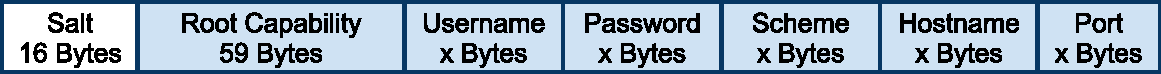
\includegraphics[scale=0.6]{KeyringFormat.pdf}
    \caption{The Keyring format. Encrypted fields are shaded in blue.}
    \label{fig:KeyringFormat}
\end{figure}

An attacker will also know some of the plaintext of the keyring. The
serialization of a capability for a writeable folder will
start with \texttt{D:RW:}, followed by 16-byte of Base32-encoded data, another
\texttt{:} and then 16 more bytes of Base32-encoded data.

\subsubsection{General Procedure}

To perform a brute force or dictionary attack on the encrypted keyring, one
must decrypt the keyring for each password guessed. The decryption involves
both key derivation with \ac{PBKDF2}, and decryption with 128-bit \ac{AES} in
\ac{ECB} mode. The \ac{PBKDF2} is a function that can be used with a
varying number of iterations, with the purpose of having a customizable way for
users to increase key strenght. Our attacks are tested on 500, 1000, 2000 and
4000 iterations.

%We verified a successful attack based on our knowledge of the
%serialization of the capability.

\subsubsection{Implemented Attacks}

We created two programs designed to crack the keyring password. The first
program, named \ac{BFDA}, was designed for a single computer, while the second
program, named \ac{CDA}, was created to perform attacks by a cluster of
cooperating computers.

Both use dictionary attacks, but the firstly mentioned is also capable of a
pure brute force attack. The source code and compiled \texttt{.jar} files for
both programs can be found in the attached CD-ROM. Implementation details are
given in Appendix \ref{ap:other}.

\subsubsection{Configuration} 

\ac{BFDA} requires Java with the \ac{JCE} and Jurisdiction Policy
files\footnote{Policy files enables Java to use stronger encryption than what
is allowed by US export law.} installed. It also depends on Java being
configured to use Bouncy Castle as its primary \ac{JCE} provider. These
prerequisites are required because the keyring is encrypted using Bouncy
Castle, as this is used by default on the Android platform.

\ac{CDA} requires almost the same configuration as \ac{BFDA}, but naturally for
each node in the cluster. Additionally, the cluster must be configured with
Apache Hadoop.

The steps we performed to set up Java with Bouncy Castle and the Jurisdiction
Policy files, are as described by \citet{jce+bc}, and the guide we used for
configuring Apache Hadoop in a Cluster using Ubuntu Server, are made by
\citet{cluster}.

\subsubsection{Hardware Specifications}

The hardware specifications for the \acl{BFDA} are given in Table
\ref{tab:hwbf}. The \acl{CDA} was executed over a cluster of Amazon \ac{EC2}
instances, of type \emph{High-CPU Extra Large Instances}. The hardware
specification for a single instance, used in the cluster attack, is given in
Table \ref{tab:hwcda}.

\begin{table}[!h]
    \centering
    \caption{Hardware Specifications for Computer Executing the \ac{BFDA}}
    \label{tab:hwbf}
    \begin{tabular}{| l | l |}
	\hline
	Product		        &HP Compaq 8100 Elite SFF PC \\
	\hline
	CPU		            &Intel(R) Core(TM) i7 CPU 860 @ 2.80GHz\\
	\hline
	Memory	            &4GB \ac{RAM}\\
	\hline
	OS		            &Ubuntu 10.10 64 bit\\
	\hline
	Kernel Version	    &Linux 2.6.35\\
	\hline
    \end{tabular}
\end{table}

\begin{table}[!h]
    \centering
    \caption{Hardware Specifications for Cluster Instances}
    \label{tab:hwcda}
    \begin{tabular}{| l | l |}
	\hline
	Instance Type       &High-CPU Extra Large Instance\\
	\hline
	CPU		            &Intel(R) Xeon(R) CPU E5410 @ 2.33GHz\\
	\hline
	CPU Architecture    &x86\_64\\
	\hline
	RAM		            &7GiB\\
	\hline
	OS		            &Ubuntu 10.10 (Maverick Meerkat)\\
	\hline
	Kernel Version	    &2.6.35-24-virtual\\
	\hline
	I/O Performance	    &High (as defined by Amazon)\\
	\hline
    \end{tabular}
\end{table}


\subsubsection{Running \ac{BFDA}}

The command used for executing a plain brute force attack with \ac{BFDA} can be
seen in Listing \ref{lst:bf}. The command for running a local dictionary attack
is seen in Listing \ref{lst:da}.

\lstset{label=lst:bf, caption=Running Local Brute Force Attack}
\begin{lstlisting}
$ java -jar BFDA.jar /path/to/keyring  \
    maximum_password_length number_of_threads
\end{lstlisting}

\lstset{label=lst:da, caption=Running Local Dictionary Attack}
\begin{lstlisting}
$ java -jar BFDA.jar /path/to/keyring \
    /path/to/dictionary number_of_threads
\end{lstlisting}

\subsubsection{Cloud Dictionary Attack with \ac{CDA}}

The cluster attack was carried out by 20 of the previously specified Amazon EC2
nodes. One instance was configured as both a Hadoop \emph{master} and
\emph{slave} node, while the 19 other instances were configured as slaves.
This was done to utilize as much as possible out of the available nodes, as the
master node performs quite a bit less computational work than the slave nodes.

Multiple scripts are needed to initiate the distributed attack.
The commands executed to start the Hadoop master and slaves, and mount up the
shared, distributed file system \ac{HDFS}, are shown in Listing
\ref{lst:hadoop}. The final command enables the Hadoop cluster to support
\emph{MapReduce}. This is necessary as the \ac{CDA} attack is implemented as a
map-reduce problem. Details about Apache Hadoop, MapReduce and the
implementation of \ac{CDA}, are given in Appendix \ref{ap:other}.

\lstset{language=bash, label=lst:hadoop, caption=Starting Hadoop Cluster with HDFS}
\begin{lstlisting}
# Start HDFS and initialize master and slave nodes
$ /path/to/Hadoop/bin/start-dfs.sh

# Start a MapReduce cluster from the master node
$ /path/to/Hadoop/bin/start-mapred.sh
\end{lstlisting}

The last requirement, before executing the attack, is to copy the
desired dictionary file and keyring into the \ac{HDFS}. Copying files from the
master node to the \ac{HDFS} is done with the command shown in Listing
\ref{lst:cpHDFS}. The attack can then be started on the master node with the
command shown in Listing \ref{lst:CDA}.

\lstset{language=bash, label=lst:cpHDFS, caption=Copying Files Into HDFS}
\begin{lstlisting}
$ /path/to/Hadoop/bin/hadoop dfs -put /path/to/file \
    /path/to/file/in/HDFS
\end{lstlisting}

\lstset{language=bash, label=lst:CDA, caption=Executing the CDA Attack}
\begin{lstlisting}
$ /path/to/Hadoop/bin/hadoop jar /path/to/CDA.jar \
    /HDFSpath/to/dictionary /HDFSpath/to/output/file \
    /HDFSpath/to/keyring number_of_slaves \
    number_of_threads_per_slave
\end{lstlisting}

%**************************************%
\chapter{Results}
\label{ch:results}
%**************************************%

\section{Client Performance}

This section displays the results of the client benchmarking and highlights the
most important results.

\subsection{Files}

The following results shows the network speed obtained when uploading and
downloading files. Table \ref{tbl:files:encrypted} shows the speed when using
the unmodified client, while Table \ref{tbl:files:unencrypted} shows the speed
obtained when using the same client but with encryption and hashing disabled.

% Kanskje en tabell her, som viser søyler med ukryptert bak og kryptert forann?
\begin{table}
  \centering
  \caption{File upload on CSV}
  \begin{tabular}{ | l | r | r |}
    \hline
    \textbf{Model}    &   \textbf{Upload}  &   \textbf{Download}   \\ \hline
    Desire   &   715 kB/s & 1,25 MB/s   \\ \hline                
    Hero     &   209 kB/s & 486 kB/s    \\ \hline 
    Computer &  27,7 MB/s & 24,9 MB/s \\ \hline
  \end{tabular}
  \label{tbl:files:encrypted}
\end{table}

\begin{table}
  \centering
  \caption{File upload/download on CSV with encryption and hashing disabled}
  \begin{tabular}{ | l | r | r |}
    \hline
    \textbf{Model}    &   \textbf{Upload}  &   \textbf{Download}   \\ \hline
    Desire & 2,62 MB/s & 2,3 MB/s \\ \hline
    Hero & 1,68 MB & 1,75 MB \\ \hline
    Computer & $\sim$70 MB/s & $\sim$70 MB/s \\ \hline
  \end{tabular}
  \label{tbl:files:unencrypted}
\end{table}


We observe that the Android devices performance for uploads is severely lower
for uploads than downloads, and that this is not the case for the computer. We
also observe that the speed with encryption and hashing enabled is severely
higher for all three devices.

\subsection{Folders}

Table \ref{tbl:folder:createblank} shows the average time it takes to create an
empty folder on the different devices. The Tables
\ref{tbl:folder:serializefolder} and \ref{tbl:folder:encryptsign} shows the
time it takes to serialize and encrypt and sign the folder respectively. These
two actions are what has to be performed every time a folder is changed, while
the creation of a blank folder is added if the content should be added to a new
folder. Table \ref{tbl:folder:verify} displays the time the devices used to
verify an existing folder, a step which is taken by the client every time a
folder is opened.

\begin{table}
  \centering
  \caption{Create a blank folder}
  \begin{tabular}{ | l | r | r |}
    \hline
   \textbf{Computer} & \textbf{HTC Desire} & \textbf{HTC Hero} \\ \hline
    81ms  &1330ms     &2060ms    \\ \hline
  \end{tabular}
  \label{tbl:folder:createblank}
\end{table}

\begin{table}
  \centering
  \caption{Serialize the contents of a folder, with n*86 bytes of data. Time in
  ms}
  \begin{tabular}{ | l | l | l | l |}
    \hline
    \textbf{n*86 bytes} & \textbf{Computer} & \textbf{HTC Desire} & \textbf{HTC Hero} \\ \hline
    500     &   &   & \\ \hline
    750     &   &   & \\ \hline
    1000    &   &   & \\ \hline
    2500    &   &   & \\ \hline     
    5000    &   &   & \\ \hline 
    7500    &   &   & \\ \hline 
    10000   &   &   & \\ \hline 
    15000   &   &   & \\ \hline 
    20000   &   &   & \\ \hline 
  \end{tabular}
  \label{tbl:folder:serializefolder}
\end{table}

\begin{table}
  \centering
  \caption{Encrypt and sign the contents of a folder with n*86 bytes of data, time in ms.}
  \begin{tabular}{ | l | l | l | l |}
    \hline
    \textbf{n*86 bytes} & \textbf{Computer} & \textbf{HTC Desire} & \textbf{HTC Hero} \\ \hline
    500     &   &   & \\ \hline
    750     &   &   & \\ \hline
    1000    &   &   & \\ \hline
    2500    &   &   & \\ \hline     
    5000    &   &   & \\ \hline 
    7500    &   &   & \\ \hline 
    10000   &   &   & \\ \hline 
    15000   &   &   & \\ \hline 
    20000   &   &   & \\ \hline 
  \end{tabular}
  \label{tbl:folder:encryptsign}
\end{table}

\begin{table}
  \centering
  \caption{Verify a folder of n*86 bytes. Time in ms}
  \begin{tabular}{ | l | l | l | l |}
    \hline
    \textbf{n*86 bytes} & \textbf{Computer} & \textbf{HTC Desire} & \textbf{HTC Hero} \\ \hline
    50      & <1    &3  & 10    \\ \hline
    100     & <1    &3  &  9    \\ \hline
    250     & <1    &3  & 11    \\ \hline   
    500     & <1    &4  & 11    \\ \hline
    750     & <1    &5  & 13    \\ \hline
    1000    &  1    &5  & 17    \\ \hline
    2500    &  3    &8  & 26    \\ \hline     
    5000    &  4    &14 & 41    \\ \hline 
    7500    &  6    &19 & N/A   \\ \hline 
  \end{tabular}
  \label{tbl:folder:verify}
\end{table}


We observe that that the slow part of folders operations are the initial key
generation and more important the serialization speed. Verification, encryption
and signing is pretty fast for all devices.

\section{Brute Force Local Keyring}
\label{sec:R:BFLK}

In Section \ref{sec:BFLK}, we tried to brute force the locally stored keyring,
by implementing and executing two different programs. The first program, named
Brute Force and Dictionary Attack (BFDA), was designed to run on a single
computer, and supports both brute force and dictionary attacks. The second
program, named Cluster Dictionary Attack (CDA), was created to run in a
computational cluster. However, the CDA attack does only support dictionary
attacks. The results for both programs are given below.

\subsection{Brute Force and Dictionary Attack (BFDA)}

With BFDA we executed both a brute force and a dictionary attack to estimate
the amount of passwords we could brute force within a second. The brute force
and dictionary attacks achieved approximately the same results. However, for
each measurement, the brute force attack turned out to achieve about 30
passwords more per seconds than the dictionary attack. This is believed to
exist due to the file reading overhead in the dictionary attack. The results
for both attacks are illustrated in Table \ref{tab:res_bf} and Figure
\ref{fig:bfres}.

\begin{table}[!h]
    \centering
    \caption{Speed results of running \acs{BFDA}}
    \label{tab:res_bf}
    \begin{tabular}{| r | r | r |}
	\hline
	\ac{PBKDF2} iterations          &Brute force attack	    &Dictionary attack	\\
	\hline
	500                             &2240 PW/s                &2240 PW/s	\\
	\hline
	1000                            &1120 PW/s                &1110 PW/s	\\
	\hline
	2000                            &570 PW/s                 &560 PW/s	\\
	\hline
	4000                            &280 PW/s                 &280 PW/s	\\
	\hline
    8000                            &140 PW/s                 &140 PW/s \\
    \hline
    \end{tabular}
\end{table}


\begin{figure}[!h]
\centering
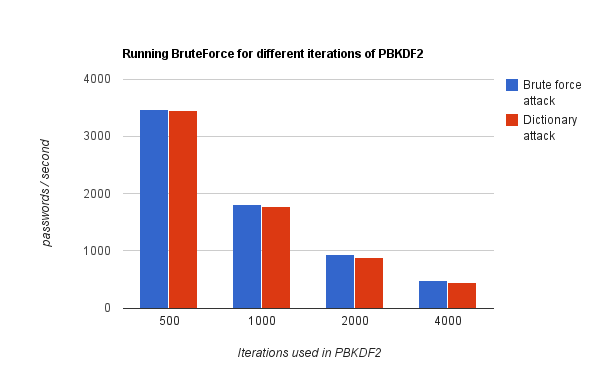
\includegraphics[scale=0.55]{bf.png}
% TODO: Cut this down!!
\caption{Results from running brute force and dictionary attacks against a local
encrypted keyring. The histogram shows how many passwords per second we were able to brute
force against different amounts of iterations used in PBKDF2.}
\label{fig:bfres}
\end{figure}

\subsection{Cluster Dictionary Attack (CDA)}

When running CDA, each node of the cluster achieved approximately the same
results as a single computer running a dictionary attack with \ac{BFDA}. We
found a small difference where the local computer achieved about 100 passwords
per second more than each instance in the cluster. With respect to difference
in CPU power between the local computer and a single cluster instance
\cite{cpubench}, this is an expected result. With 20 nodes in the cluster we
were able to brute force around 35 000 passwords per second, given
\emph{PBKDF2} with 1000 iterations.

%**************************************%
\chapter{Discussion}
\label{ch:discussion}
%**************************************%
%\section{Complexity}
% Hvordan vi lagrer filer
% Lagring av nøkler
% Hvordan direktorier fungerer
% Hvordan vi deler

%Vår løsning VS relatert research og existing solutions

%\subsection{Keys}
%Type of keys, what distribution scheme was chosen
%\subsection{Files}

%\subsection{Folders}

%\subsection{Sharing}

\section{Cryptographic Scheme}
%What is/is not used from TAHOE?

\section{Implementation}
This section will discuss and deal with the different choices taken to fulfill
the implementation of the cryptographic scheme. We will start by discussing the
use case we chose to implement. We will further analyse our choice of key
distribution and look at alternative solutions. The section will end by
discussing the most important cryptographic primitives chosen and utilized in our
implementation.

\subsection{Choice of Use Case}

\subsection{Choice of Key Distribution}
\label{sec:DI:keydist}
%Describe possible key distributions schemes
%Argue why we chose our scheme
\subsection{Choice of Cryptographic Primitives}

\section{Performance}
% 1 mappe med 100 filer i, tar ikke mye lenger tid å åpne enn en mappe med 3
% filer i
\subsection{Sources of Error}

\section{Security}
% Hvordan angripe?
% ACL lag bare ekstra sikkerhet, man kan ikke cracke noe uten keyen!
This thesis is written with the basis that we are hiring storage from an
untrusted provider, and the security of the application should primarily
reflect that. With this starting point we can assume that all data stored on
the server is obtainable by the provider.

\subsection{Passive Attacks}
% Avhengig av cryptographic primitives
% Confidentiality den største utfordringen
% Her trengs det gode kilder
The provider will have access to all data on the server, and also know what
data stored is part of files and what is part of folders. The confidentiality
of both files and folders relies primarily on the symmetric cipher used to
encrypt the data. But for folders one can obtain this key if one manages to
obtain the asymmetric private key belonging to the folder. In other words a
folder is attackable both trough the asymmetric and the symmetric cipher used.
If the confidentiality of a folder is breached it will additionally enable the
attacker to decrypt all of the corresponding sub-folders and files. In contrast,
cracking the confidentiality of a file will only compromise that specific file. It is
also important to note that users will use a root folder which any other file
or folder relies on, if the confidentiality of this folder is breached, all
files are effectively compromised.

\subsubsection{Brute Force Local Keyring}
The confidentiality of the root folder can be breached by brute forcing a user's
locally stored keyring. This was experienced in Section \ref{sec:BFLK}. From the
results in Section \ref{sec:R:BFLK} and Figure \ref{fig:bfres}, we noticed
that the choice of iterations in \emph{PBKDF2} were conclusive to the efficiency of a
brute force attack against the local keyring. By doubling the number of
iterations in \emph{PBKDF2}, the efficiency of a brute force attack would decrease by
half of it's value. The \emph{PBKDF2} standard, written by RSA Laboratories in 1999 \cite{PBKDF2std},
recommends the minimum number of iterations to be 1000. With 1000 iterations in
\emph{PBKDF2} we were able to achieve a brute force efficiency around 1800 passwords
per second for a single computer, and 35 000 passwords per second running the
CDA attack on 20 Amazon EC2 high-CPU extra large instances. Given a password
with length 5 and containing only small letters, the CDA attack will use 5
minutes and 39 seconds to check all possible values. By using a cluster of 200
nodes the CDA attack is able to crack a similar password of length 6 within 14 minutes
and 42 seconds in worst case.\\

\noindent It is important to notice that both CDA and \ac{BFDA} programs were
written in Java. With this in mind, it is reasonable to believe
that general performance can be improved by using lower-layer
programming languages, such as C, to implement the attacks. Another way to
increase performance is to design both attacks to run on \ac{GPU}s rather than CPUs.\\

\noindent Regarding CDA, the use of cloud computing to execute a brute force
attack is not a new idea \cite{bfpgp, rothsha, rothwpa}. Newly on Black Hat DC 2011, a
security researcher named Thomas Roth, showed that it was possible to brute
force WPA passwords with a speed of 47 000 passwords per second on a single EC2
cluster GPU instance \cite{rothwpa}. Amazon allows a user to execute up to 8
cluster GPU instances, without the need of a special request. This indicate that
anyone can crack WPA passwords at almost 400 000 passwords per second, and that
Amazon can achieve even higher and unknown speed for WPA password cracking. With
this in mind, we should consider that our own keyring can be subject to a lot
more efficient brute force attacks compared to our own findings.\\

\noindent To reduce vulnerability from plain brute force attacks, we decided to
use 4000 iterations in \emph{PBKDF2}. In addition, we designed the Cloud Storage Vault
to force users to utilize more advanced and sophisticated passwords. Password
requirements for the Cloud Storage Vault are given below:

\begin{itemize}
\item Password length >= 9.
\item Password must include at least one capital letter, one small letter and
one number.
\end{itemize}

\noindent With the password requirements above and with 4000 iterations in
\emph{PBKDF2}, it will
be extremely hard to perform a plain brute force attack against the local
keyring. Figure \ref{fig:bfres} indicates that when using \emph{PBKDF2} with 4000
iterations, the local test computer running \ac{BFDA} is only able to check
around 400 passwords per second. Given a cluster of 200 such computers, it will
take 2683 years on average to brute force a password using the syntax above
and a length of 9.\\

\noindent Even though the keyring is secured against a plain brute force attack, it is
still, to a certain degree,  vulnerable to a dictionary attack.

\subsubsection{RSA attacks}

\subsubsection{AES attacks}

\subsection{Active attacks}
% MITM - Dersom vi f.eks. skrur av SSL-laget
% Innside attacker - hos Amazon


\subsection{Terminal security}
% What happens if someone steals a terminal
% OR install some backdoor/torjan etc?
Given enough users, at some point there will be a users who looses his
terminal, for instance a mobile phone, a terminal might also be broken into
without the users knowledge.


\section{Additional Features}
% Ting vi ikke har lagt inn
% - Cascading deletes? Loops.
% - Hvem 'eier' en directory
% - Garbage collection? (vanskelig)


%**************************************%
\chapter{Conclusion and Future Work}
\label{ch:conclusion}
%**************************************%

\section{Compared with Other Solutions}
% BibTeX bibliography lives in external file
\bibliographystyle{unsrtnat}
\bibliography{references}
% TODO: Can we fix references in order of apperance?

%**************************************%
\appendix
\appendixpage
\addappheadtotoc
%**************************************%
%**************************************%
\chapter{Other Relevant Implementations}
\label{ap:other}
%**************************************%

This chapter will study implementation details from applications that were
created, but not a part of the thesis' main topic. Applications considered are
Brute Force and Dictionary Attack (BFDA) and the Cluster Dictionary Attack (CDA).

\section{Brute Force and Dictionary Attack}

\emph{\ac{BFDA}} includes a plain brute force attack and a dictionary attack against
a users encrypted keyring. Details about the implementation follows.

\subsection{Implementation Details}

\ac{BFDA} is written in Java and utilize the \texttt{javax.crypto} library with Bouncy
Castle version 1.34 as JCE provider to decrypt the encrypted keyring. The
Bouncy Castle JCE provider seems to be necessary as Android 2.2 uses it by
default to encrypt the keyring. To enable \emph{PBKDF2} before decryption, \ac{BFDA}
utilize a \emph{PBKDF2} Java library \cite{pbkdf2}.

The program is divided into two functions, named \texttt{bruteForceAttack} and
\texttt{dictionaryAttack} that correspondingly executes a brute force and
dictionary attack. The \texttt{bruteForceAttack} function is shown in Listing
\ref{lst:bffunc}.

\lstinputlisting[language=java, label=lst:bffunc, caption=bruteForceAttack
function]{listings/bruteForceAttack.java}

\texttt{bruteForceAttack} starts a number of \texttt{BruteForceThread} threads.
The function continues after all \texttt{BruteForceThreads} are initialized and
ready to start their task. It then enters a while-loop, which executes a
\texttt{pushWord} function for each iteration.

The task of \texttt{pushWord} is to simply create and push all possible words
of a given length onto a stack of words. The length of the words to push are
given by its integer argument. The whole attack is based on letting the main
thread create and push words onto a stack, while the \texttt{BruteForceThreads} are
pulling words from the stack. When a word is pulled from the stack, it is
subject to \emph{PBKDF2}, where the result is used to decrypt the ciphertext. If
decryption results in a given plaintext, the password is found.

The \texttt{dictionaryAttack} function is shown in Listing \ref{lst:dafunc}.

\lstinputlisting[language=java, label=lst:dafunc, caption=dictionaryAttack
function]{listings/dictionaryAttack.java}

\texttt{dictionaryAttack} reads an input dictionary file into a
\texttt{BufferedReader}. It then starts a given number of
\texttt{DictionaryThreads}. The \texttt{DictionaryThreads} will read from the
\texttt{BufferedReader} in a synchronized way. When a word is read from a
\texttt{DictionaryThread} it will be subject to \emph{PBKDF2}, where the result is
used to decrypt the ciphertext. If decryption results in a given plaintext, the
password is found.

\section{Cluster Dictionary Attack}

The \ac{CDA} is written in Java, and is built around the same procedure as the
dictionary attack in \ac{BFDA}. However, the difference lays in the cooperation
of multiple computers. To enable a cluster of computers to cooperate, we used
the following environment.

\subsection{Environment}

The environment is based upon a software framework from Apache called
\emph{Hadoop}. The main functionality of Hadoop is described below.

\subsubsection{Apache Hadoop}

Apache Hadoop makes it possible for multiple machines to cooperate
and run computational work together. Hadoop also provides a distributed filesystem
\ac{HDFS}, that can store data across multiple cooperating machines \cite{hadoop}. The
computational work in Hadoop is organized and distributed using \emph{MapReduce}.

\paragraph{MapReduce} MapReduce is a programming paradigm introduced by Google.
It is designed to process and generate large sets of data using a cluster of
machines \cite{mapred}. 

In MapReduce, a large set of input data is divided into multiple key/value
pairs. The key/value pairs are further distributed to multiple MapReduce tasks
running on multiple machines. 

A MapReduce task is divided into a \emph{mapper} and a \emph{reducer}. The task
of a mapper is to perform an operation on a key/value pair and return a
key/value pair as a result to the reducer. The reducer collects key/value pairs
from multiple mappers and combine the results into one or more output files.

\subsection{Implementation Details} 

The \ac{CDA} attack is implemented as a MapReduce problem, with a large
dictionary file as the data input set. The dictionary is split into separate
key/value pairs, where each value is a single line in the dictionary and the
key corresponds to the line's offset within the dictionary.

The key/value pairs are handled by a map function implemented in
\texttt{CDAMapper}. The
map function has the responsibility of checking every word on a single
dictionary line. Each line in the dictionary should contain a certain amount of
words. This is to enable the map function to run multiple threads at the same
time, where each thread checks one or more words. With multiple threads, the
attack is able to utilize more \ac{CPU} power for each running machine in the
cluster. A detailed view of the map function, is given in Listing
\ref{lst:mapfunc}.

\lstinputlisting[language=java, label=lst:mapfunc, caption=Mapper function in
CDAMapper]{listings/mapper.java}

When receiving a key/value pair, the map function first splits the input line
into an array of words called line. It then creates a given number of
\texttt{DictionaryThread} threads and serves each thread a sub array of words from the
line array. Each \texttt{DictionaryThread} will check all of its incoming words similar
to the \texttt{DictionaryThread} in BFDA. If the correct password is found, the
password will be written to the \texttt{sysout} folder on the machine where the mapper is
running.

A class named \texttt{Processor} initializes the \ac{CDA} attack by configuring
the mapper and reducer tasks. The number of mappers is set equal to the number
of nodes used in the cluster. This is to ensure that each machine only runs one
mapper at a time. The number of reducers are set to zero, because their
behavior in MapReduce is not needed.

\paragraph{Notice} The for-loop at Line 10 in Listing \ref{lst:mapfunc}
requires the number of words per line, in the dictionary, to be equal to a
multiple of the number of threads in use. It is recommended that the input
dictionary follows this requirement. 

In this occasion, we have created a Bash script, named \texttt{dictmaker.sh},
that changes a regular dictionary into an $N$ words-per-line dictionary. The
script can be found on the attached CD-ROM.

%**************************************%
\chapter{Attachments}
\label{ap:attachments}
%**************************************%

This thesis comes with two available attachments -- one digitally uploaded to
the DAIM system\footnote{\url{http://daim.idi.ntnu.no/}}, and one physical DVD.

\section{Electronic Attachment}

The electronic attachment, uploaded to
DAIM, consists of the following files
and directories:

\begin{description}
  \item[Application] All files and source code to the proof of concept system,
    i.e. the background library, server and client.
  \item[Report] All files that is used to create this report, including images
    and tables.
  \item[Other] Scripts and raw data from the experiments.
\end{description}

\section{Attached DVD}

All the source code generated while working on this thesis, including the
source code for the proof of concept client code, can be found on an attached
DVD. In addition, all files related to the writing of this document, including
images and most of the references, are also included on the same DVD.

\end{document}
